\documentclass[]{politex}
% ========== Opções ==========
% pnumromarab - Numeração de páginas usando algarismos romanos na parte pré-textual e arábicos na parte textual
% abnttoc - Forçar paginação no sumário conforme ABNT (inclui "p." na frente das páginas)
% normalnum - Numeração contínua de figuras e tabelas 
%	(caso contrário, a numeração é reiniciada a cada capítulo)
% draftprint - Ajusta as margens para impressão de rascunhos
%	(reduz a margem interna)
% twosideprint - Ajusta as margens para impressão frente e verso
% capsec - Forçar letras maiúsculas no título das seções
% espacosimples - Documento usando espaçamento simples
% espacoduplo - Documento usando espaçamento duplo
%	(o padrão é usar espaçamento 1.5)
% times - Tenta usar a fonte Times New Roman para o corpo do texto
% noindentfirst - Não indenta o primeiro parágrafo dos capítulos/seções
	
% ========== Packages ==========
\usepackage{xcolor}
\usepackage{hyperref}
\usepackage[section]{placeins}
\def\sectionautorefname{}
\def\subsectionautorefname{}
\def\subsubsectionautorefname{}
\def\tableautorefname{Tabela}
\def\equationautorefname{}
\newcommand\myworries[1]{\textcolor{red}{#1}}
\newcommand\cmrtext[1]{\fontfamily{cmr}\selectfont {#1}\normalfont}
\usepackage{array}
\newcolumntype{L}[1]{>{\raggedright\let\newline\\\arraybackslash\hspace{0pt}}m{#1}}
\newcolumntype{C}[1]{>{\centering\let\newline\\\arraybackslash\hspace{0pt}}m{#1}}
\usepackage{chngcntr}
\counterwithout{equation}{chapter}

%\newcommand{\fonte}[1]{{\small Fonte}: {#1}} 
\usepackage{physics}
\usepackage[utf8]{inputenc}
\usepackage{amsmath,amsthm,amsfonts,amssymb}
\usepackage{graphicx,cite,enumerate}
\graphicspath{ {./images/} }
\usepackage{fontspec}
\setmainfont{Arial}
\delimitershortfall=-1pt

% ========== Language options ==========
\usepackage[brazil]{babel}
%\usepackage[english]{babel}


% ========== ABNT (requer ABNTeX 2) ==========
%	http://www.ctan.org/tex-archive/macros/latex/contrib/abntex2
\usepackage[alf, versalete, abnt-emphasize = bf]{abntex2cite}

% Forçar o abntex2 a usar [ ] nas referências ao invés de ( )
%\citebrackets{[}{]}

% ========== Opções do documento ==========
% Título
\titulo{Análise Numérica da Difusão de Nitrogênio durante a Nitretação dos Aços}

% Autor
\autor{Julia Moraes}


% Orientador / Coorientador
\orientador{Prof. Dr. Eduardo Franco de Monlevade}

% Tipo de documento
\tcc{Engenharia de Materiais}
%\dissertacao{Engenharia Elétrica}
%\teseDOC{Engenharia Elétrica}
%\teseLD
%\memorialLD

% Departamento e área de concentração
%\departamento{Nome do departamento}
%\areaConcentracao{Área de concentração}

% Local
\local{São Paulo}

% Ano
\data{2019}


\begin{document}
% ========== Capa e folhas de rosto ==========
\capa
%\falsafolhaderosto
%\folhaderosto

\chapter{tmp}
\par \myworries{colocar a legenda da figura embaixo}

\myworries{[23] nitriding can be considered as a one-d problem because...
}
% ========== Listas (opcional) ==========
\listadefiguras
\listadetabelas

% ========== Sumário ==========
\sumario


% ========== Elementos textuais ==========
\chapter{Introdução}

\myworries{//O objetivo é buscar entender o perfil obtido (plato...) e a velocidade ---
 criar um modelo simplessssss e verificar a validade do mesmo}

\chapter{Revisão Bibliográfica}
\section{Difusão}
\label{sec:difusao}
	A difusão é um processo de transporte de matéria, no qual a matéria é transportada de uma posição no sistema para outro através de movimentos moleculares aleatórios \cite{crank1979mathematics}. Para que exista difusão é necessária uma diferença de potencial químico, que atua como força motriz para o fenômeno, um exemplo é o gradiente de concentração do átomo no meio dado pela eq.(\ref{eq:gradC}) [g/cm$^4$]. 

\begin{equation} \label{eq:gradC}
\nabla C = \pdv{C}{x}e_x + \pdv{C}{y}e_y + \pdv{C}{z}e_z
\end{equation}

Para quantificar esse processo, define-se um fluxo de difusão, que corresponde à massa difundida por unidade de tempo através de uma área unitária perpendicular à direção do movimento de massa. Quando a difusão ocorre em estado estacionário, isto é, a concentração do elemento não varia com o tempo e consequentemente o fluxo também é constante, o fluxo de difusão de uma determinada espécie química pode ser relacionado à sua diferença de concentração como na eq.(~\ref{eq:primeiraLeiFick}), também conhecida como primeira lei de Fick. O fluxo de difusão ocorre na direção contrária à do gradiente de concentração, ou seja, os átomos se movimentam das regiões de maior concentração para as de menor concentração.

\begin{equation} \label{eq:primeiraLeiFick}
J = -D\nabla C = -D(\pdv{C}{x}e_x + \pdv{C}{y}e_y + \pdv{C}{z}e_z)
\end{equation}

	Na primeira lei de Fick, J representa o fluxo de difusão [g/cm$^2$.s] e D é o coeficiente de difusão [cm$^2$/s]. Considerando o caso unidimensional e dado que em estado estacionário a concentração não varia com o tempo, também não há variação com a posição, portanto $dC/dx$ é constante e $C(x)$ é uma função linear de x, como mostra a Figura \ref{fig:primeiraLei}. \par
	
	\begin{figure}[ht]
	\caption{Perfil de concentração correspondente à primeira lei de Fick}
	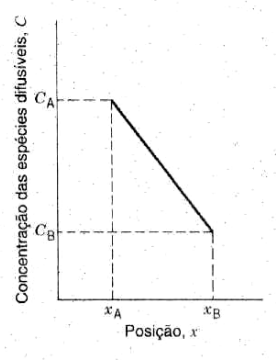
\includegraphics{primeiraLei}
	\label{fig:primeiraLei}
	\centering
	\fonte{Callister, 1940}
	\end{figure}

	Para o caso de difusão em regime não estacionário, tanto o gradiente de concentração, quanto o fluxo variam com o tempo. Nesse caso, utilizando a equação de conservação das espécies químicas e a Primeira Lei de Fick é possível definir a Segunda Lei de Fick dada pela eq.(\autoref{eq:segundaLeiFick}) que relaciona a variação da concentração da espécie química no tempo com sua variação de concentração no espaço. \par

\begin{equation} \label{eq:segundaLeiFick}
 \pdv{C}{t} = \nabla.(D\nabla C)
\end{equation}

	Quando condições de contorno são identificadas para situações reais é possível obter uma solução para essa equação. Uma forma de encontrar uma solução para a Segunda Lei de Fick é através da utilização de uma variável de similaridade, que consiste em reduzir o número de variáveis independentes para apenas uma variável, que depende das originais. A seguir será destacado uma possível solução retirada de \cite{notas-modelos}. \par
	Considerando que o teor do átomo que se difunde é constante na superfície ao longo do tempo, que o transporte ocorre sob condições isotérmicas, com coeficiente de difusão constante, em um corpo semi infinito, para o caso unidimensional, seguem as condições necessárias para se encontrar uma solução. Seja c$_i$ a concentração inicial no interior do substrato e c$_s$ a concentração na superfície.\par
\myworries{melhorar essa deducao}
\begin{center} 
	Condição inicial : $C(x,t=0) = c_i$ \\
	Condições de contorno (condições de Dirichlet): 
	\begin{math}
  		\left\{
    	\begin{array}{l}
      		C(x=0,t>0) = c_s\\
      		C(x\rightarrow \infty, t>0) = c_i
    	\end{array}
  		\right.
	\end{math}
\end{center}

A eq.(\ref{eq:segundaLeiFick}) para uma dimensão, com D constante é:

\begin{equation} \label{eq:segundaLeiFickUmD}
 \pdv{C}{t} = D\pdv[2]{C}{x}
\end{equation}

Definição da variável de similaridade $\eta$:

\begin{center}
	\begin{math}
		\eta = \eta(x,t) \Rightarrow \eta = Axt^m
		\left\{
    		\begin{array}{l}
      			C(\eta\rightarrow \infty) = c_i\\
      			C(\eta=0) = c_s
    		\end{array}
		\right.
	\end{math}
\end{center}

Aonde $A$ e $m$ são constantes.
Realizando a mudança de variável obtém-se:
\begin{equation} \label{eq:solA}
 \pdv{C}{t} = \frac{dC}{\eta}\pdv{\eta}{t} = \frac{dC}{d\eta}mAxt^{m-1} = \frac{dC}{d\eta}m\eta t^{-1}
\end{equation}

\begin{equation} \label{eq:solB}
 \frac{dC}{dx} = \frac{dC}{d\eta}\pdv{\eta}{x} = \frac{C}{\eta}At^m
\end{equation}

\begin{equation} \label{eq:solC}
 \frac{d^2C}{d^2x} = \pdv{}{x}\pdv{C}{x} = \pdv{}{x}(\frac{dC}{d\eta}At^m) = \pdv{}{x}(\frac{dC}{d\eta})At^m = \frac{d}{d\eta}(\frac{dC}{d\eta})\frac{d\eta}{dx}At^m = \frac{d^2C}{d\eta ^2}A^2t^{2m}
\end{equation}

Substituindo as equações \autoref{eq:solB} e \autoref{eq:solC} na equação \autoref{eq:segundaLeiFickUmD}:

\begin{equation} \label{eq:solD}
 \frac{dC}{d\eta}m\eta t^{-1} = D \frac{d^2C}{d\eta ^2}A^2t^{2m} \Rightarrow \frac{d^2C}{d\eta ^2} - \frac{mt^{-1}}{DA^2t^{2m}}\eta \frac{dC}{d\eta} = 0 
\end{equation}

Considerando as constantes arbitrárias a seguir:
\begin{gather*}		
	\frac{t^{-1}}{t^{2m}} = 1 \Rightarrow m = -\frac{1}{2} \\
	4DA^2 = 1 \Rightarrow A = \frac{1}{\sqrt{4D}}
\end{gather*}	

Substituindo na equação \autoref{eq:solC}:
\begin{equation} \label{eq:solE}
 \frac{d^2C}{d\eta ^2} + 2\eta \frac{dC}{d\eta} = 0
\end{equation}

Aonde $\eta = Axt^m = \dfrac{1}{\sqrt{4D}}xt^{-1/2} = \dfrac{x}{2\sqrt{Dt}}$.

Segue a resolução matemática:

\begin{gather*}		
	\varepsilon = \frac{dC}{d\eta} \Rightarrow \frac{dC}{d\eta} + 2\eta\varepsilon = 0 \\
	\frac{dC}{d\eta} = -2\eta\varepsilon \Rightarrow \int\frac{d\varepsilon}{\varepsilon} = \int -2\eta d\eta + \lambda \Rightarrow ln\varepsilon = -\eta^2 + \lambda \Rightarrow \frac{dC}{d\eta} = \varepsilon = \lambda'e^{-\eta^2} \\
	\int_{c_s}^{c} dC = \int_{0}^{\eta} \lambda'e^{-\eta^2} d\eta 
\end{gather*}	

\begin{equation} \label{eq:solF}
	c - c_s =  \lambda'\int_{0}^{\eta} \eta'e^{-\eta^2} d\eta 
\end{equation}

Utilizando a seguinte condição de contorno: $C(\eta\rightarrow \infty) = c_i$ 

\begin{gather*}	
	c_i - c_s = \lambda\int_{0}^{\infty} \lambda'e^{-\eta^2} d\eta  \\
	\int_{0}^{\infty} \lambda'e^{-\eta^2} d\eta  = \frac{\sqrt{\pi}}{2} \Rightarrow 			\lambda = (c_i - c_s)\frac{2}{\sqrt{\pi}}
\end{gather*}

Substituindo $\lambda$ em \autoref{eq:solF}:
\begin{equation} \label{eq:solG}
	\frac{c - c_s}{c_i - c_s} = \frac{2}{\pi} \int_{0}^{\eta} \eta'e^{-\eta^2} d\eta   
\end{equation}
Para $\eta = \dfrac{x}{2\sqrt{Dt}}$.

A expressão $ \frac{2}{\pi} \int_{0}^{\eta} \eta'e^{-\eta^2} d\eta $ é a função erro $erf(\eta)$ e  $1 - erf(\eta)$ é seu complementar $erfc(\eta)$. Logo, chega-se que 

\begin{equation} \label{eq:solFinal}
	1 - \frac{c - c_s}{c_i - c_s} = \frac{c - c_i}{c_s - c_i} = 1 - erf(\eta) = erfc(\eta) \Rightarrow c = c_i + (c_s - c_i) erfc(\eta)
\end{equation}

\par O perfil de concentração para regime não estacionário ao longo do tempo está representado na Figura \ref{fig:segundaLei}.

\begin{figure}[ht]
	\caption{Perfil de concentração correspondente à segunda lei de Fick}
	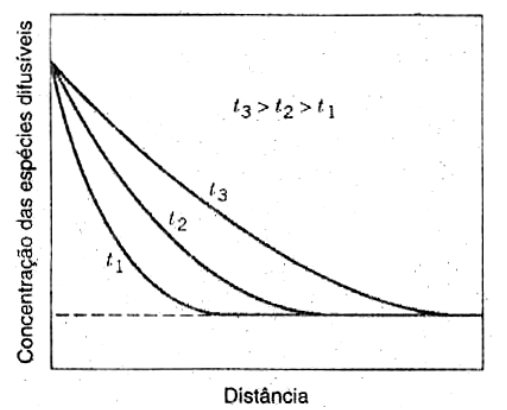
\includegraphics[width=80mm,scale=0.5]{segundaLei}
	\label{fig:segundaLei}
	\centering
	\fonte{Callister, 1940}
\end{figure}

\par
	A variável $\sqrt{Dt}$ é chamada de distância de difusão e representa a distância percorrida por um átomo com coeficiente de difusão D, após um tempo t. Considerando a solução encontrada (eq \autoref{eq:solFinal}), para c =  $c_x$ = cte, tem-se

$$\frac{c_x - c_s}{c_i - c_s} = 1 - erf(\frac{x}{2\sqrt{Dt}}) = cte \Rightarrow erf(\frac{x}{2\sqrt{Dt}}) = cte \Rightarrow \frac{x}{2\sqrt{Dt}} = cte$$

\begin{equation} \label{eq:difdist}
		\therefore x \propto  \sqrt{Dt}
\end{equation}


\subsection{Mecanismos de difusão em sólidos}
	Existem diferentes mecanismos de difusão, isto é, diferentes formas em que um átomo pode mudar de posição em um reticulado cristalino. Em geral, em sólidos cristalinos com reticulados bem definidos, a difusão ocorre na forma de movimentos atômicos. A probabilidade de um átomo se deslocar em uma determinada direção e uma dada distância é função da microestrutura do material e das forças interatômicas \cite{glicksman2000diffusion}.
	
	As direções possíveis para o movimento aleatório em materiais cristalinos são limitadas pela sua cristalografia, mais especificamente são as direções paralelas aos vetores que ligam pontos vizinhos do reticulado ou espaços intersticiais.
	Diferentes mecanismos de difusão podem existir mutuamente sendo que alguns fatores determinam qual será mais frequente, como por exemplo o tamanho do átomo com relação ao átomo hospedeiro. De forma geral, para que ocorra mudança de posição de um átomo é necessário que haja uma posição livre adjacente a sua posição atual e o mesmo deve possuir energia suficiente para quebrar as ligações químicas existentes com seus vizinhos e causar uma distorção no reticulado durante seu deslocamento. \par

Os principais mecanismos de difusão são:
\subsubsection{Difusão por lacuna}
A difusão por lacuna ocorre quando um átomo se desloca de uma posição normal do reticulado para uma posição vazia, uma lacuna, que em si é um defeito presente na rede cristalina. Quanto maior a quantidade desses defeitos maior a possibilidade de difusão por esse mecanismo \cite{callister2007materials}. Ele predomina no caso de difusão de átomos substitucionais e até mesmo na autodifusão. Nessa difusão ocorre uma distorção do reticulado quando o átomo muda de posição, o que torna necessário que haja uma energia mínima envolvida nesse processo. A Figura \ref{fig:dif-lacuna} esquematiza esse mecanismo.

\begin{figure}[ht]
	\caption{Esquema para explicar difusão por lacuna}
	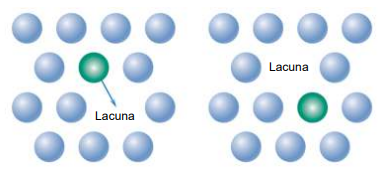
\includegraphics[width=80mm,scale=0.5]{dif-lacuna}
	\label{fig:dif-lacuna}
	\centering
	\fonte{Adaptado de Callister, 1940}
\end{figure}


\subsubsection{Difusão intersticial}
	Nesse mecanismo o átomo se desloca de uma posição intersticial do reticulado para outra que se encontra vazia. É importante que o átomo possua energia suficiente para deslocar o reticulado entre as duas posições, pois para alcançar o outro interstício ele precisa superar as forças de repulsão do reticulado no plano que separa os dois interstícios. Quando o átomo se encontra entre duas posições fala-se que ele está no estado ativado, que é o ponto em que ele possui maior energia. Caso não haja energia cinética e momento suficiente o átomo retorna à posição de origem \cite{glicksman2000diffusion}. 
	Esse tipo de difusão é relevante para átomos que apresentam raios menores que os dos átomos que constituem a rede cristalina. A energia do átomo em função da sua posição é mínima quando ele se encontra em um interstício e máxima quando se encontra no estado ativado. Esse costuma ser um mecanismo mais rápido que outros pois a ocorrência de interstícios é maior que a de lacunas e os átomos menores conseguem se desocar com mais facilidade \cite{murty2013introduction}.
	
	\begin{figure}[ht]
	\caption{Esquema para explicar difusão intersticial}
	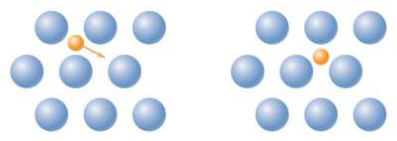
\includegraphics[width=80mm,scale=0.5]{dif-intersticio}
	\label{fig:dif-insterticial}
	\centering
	\fonte{Adaptado de Callister, 1940}
\end{figure}
	
%\myworries {pegar uma imagem do murty?}
	
\subsubsection{Difusão em contorno de grão}
A difusão em contorno de grão é mais rápida que os outros mecanismos (assim como ocorre com a difusão em outros defeitos como discordâncias e superfícies externas). Isso se deve ao fato que o espaço disponível nessas regiões é maior do que aquele no volume do reticulado cristalino. Mas pode se tornar pouco significante dado que a seção transversal das áreas é relativamente menor que comparada ao interior do material. 

\subsection{Fatores que influenciam na difusão}
	A difusão depende da espécie do átomo em difusão e da espécie que constitui o meio em que ele se difunde. Isso ocorre pois o tamanho do átomo e o espaço que ele tem para se locomover influenciam na difusão, assim como a interação química entre ambos, pois esses fatores afetam qual será o mecanismo predominante da difusão ~\cite{callister2007materials}. A temperatura também influencia a difusão à medida que um aumento da temperatura aumenta a vibração dos átomos e consequentemente sua mobilidade e difusão, além de aumentar também a concentração de lacunas. 
	
	Dada a influência dos diferentes fatores na difusão, como a espécie em difusão, o material hospedeiro e a temperatura, o Coeficiente de Difusão D pode ser dado pela equação \autoref{eq:coeficiente-de-dif}.
\begin{equation} \label{eq:coeficiente-de-dif}
	D = D_0 \ {e^{\frac{-E_A}{RT}}}		
\end{equation}

Os termos das equação \autoref{eq:coeficiente-de-dif} estão listados a seguir:

$D_0$ : constante pré-expnencial independente da temperatura [$m^2/s$]

$E_A$ : energia de ativação para difusão [$J/mol$ ou $eV/$átomo]

$R$ : constante universal dos gases [$8,31 J/mol.K$ ou $8,62 10^{-5} eV/$átomo$.K$]

$T$ : temperatura absoluta [$K$]

Também é possível utilizar a constante de boltzmann $k_B$ [$J/mol$] no lugar da constante universal dos gases se a energia de ativação estiver em $Joule$.

A energia de ativação é a energia necessária para movimentar um mol de átomos por difusão, quanto maior for, menor será o coeficiente de difusão D. Com relação à temperatura, pode-se observar que quanto mais elevada, maior será o termo exponencial, logo maior o coeficiente de difusão.

\section{Nitretação}
	A nitretação é um processo de tratamento térmico que promove a adição de nitrogênio através da superfície de metais através da difusão. Esse tratamento é frequentemente utilizado para melhorar as propriedades mecânicas do material, em especial, a sua dureza. No caso de aços austeníticos, também é utilizado para aumentar a resistência ao desgaste sem prejudicar a resistência à corrosão \cite{baranowska2010importance}.
	 Aplicações importantes desse processo são materiais da indústria petrolífera, que são utilizados para a extração de petróleo.
	 Existem diferentes métodos de nitreteção, eles podem ser divididos em três categorias: nitreção à gás,  nitretação líquida e nitretação por plasma.
	 
\subsection{Nitretação à gás}
	A nitretação à gás utiliza um gás rico em nitrogênio (como amônia), que se dissocia ao entrar em contato com a peça que é aquecida e então consegue se difundir através da superfície, criando uma camada nitretada que possui maior dureza \cite{zimmermannnitretaccao}.   
	Esse proesso permite controle do potencial químico do nitrogênio através do fluxo do gás, permite também realizar o tratamento em peças de grande volume e possui um custo baixo comparado a outros métodos. Porém, é sensível às condições da superfície e pode ser necessário fazer um tratamento prévio da superfície para remover camadas de óxidos, por exemplo.
	 
\subsection{Nitretação líquida}
	Para a nitreção líquida, utiliza-se um banho de sal que contém nitrogênio (como por exemplo cianetos). O nitrogênio difunde para o interior da peça quando esta é mergulhada no banho em temperaturas entre 550 e 570°C. Posteriormente a peça é retirada, lavada e esfriada \cite{zimmermannnitretaccao}. 
	Em geral esse método é rápido, com duração de aproximadamente 4 horas e simples de ser executado pois basta mergulhar a peça no banho. Apresenta como desvantagem a toxidade dos sais utilizados, o que aumenta os custos relativos a segurança e leis ambientais.
	
\subsection{Nitretação por plasma}
	O método de nitretação por plasma consiste na utilização de plasma de nitrogênio para promover a adição dessa espécie no material da peça. 
	O plasma é um estado da matéria que ocorre quando um gás é ionizado, isto é, os seus átomos perdem ou ganham elétrons, o que o torna condutor elétrico. Esse estado pode ser alcançado quando a substância é exposta à temperaturas suficientemente altas ou a um campo eletromagnético intenso. Na nitretação o plasma utilizado é uma mistura de átomos de nitrogênio e hidrogênio ou gás nitrogênio puro.
	Para a preparação da superfície, camadas superficiais podem ser removidas por sputtering, que consiste da remoção de átomos devido à colisão dos íons no material, que podem colidir com energia maior que a energia de ligação desses átomos.
	 Esse processo permite um controle da espessura e da camada nitretada, requer uma temperatura de tratamento menor que outros métodos - com valores entre 320 e 550°C, apresenta tempo de trabalho menor que outros processos e consequentemente representa uma economia no consumo de gás e de energia \cite{zimmermannnitretaccao}. 
	Uma grande vantagem desse método é que ele não promove a formação de nitretos de cromo como alguns outros, o que o torna interessante para aplicação em aços inoxidáveis.
	
\section{Aços}
	Aços são ligas metálicas constituídas essencialmente de ferro e carbono, com teor de carbono entre 0,008 e 2,11\% em peso. A microestrutura dos aços varia com o teor de carbono presente e também com os elementos de liga e suas quantidades. Os principais elementos de liga utilizados em aços são cromo, molibdênio, níquel e nitrogênio. Eles definem diferentes propriedades da liga e também influenciam na estabilização de diferentes microestruturas desse material. \par
	As principais estruturas cristalinas dos aços segundo o diagrama de fases ferro-carbono são a ferrita (ferro $\alpha$) de estrutura CCC, a austenita (ferro $\gamma$) de estrutura CFC e a ferrita $\delta$ também CCC. A cementita (Fe$_{3}$C) é um carbeto de ferro que se forma para concentrações de carbono superiores a 6,70\% em peso. Na Figura \ref{fig:diagrama-fases-fe-c} está representado um diagrama de fases para a liga ferro-carbono, que relaciona as concentrações de carbono para uma dada temperatura com a fase correspondente no equilíbrio.
	
\begin{figure}[ht]
	\caption{Diagrama de Fases Fe-C}
	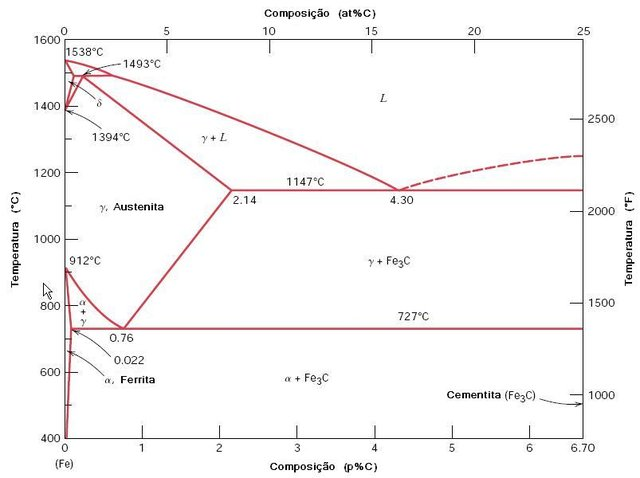
\includegraphics[width=0.8\textwidth]{diagrama-fases-fe-c}
	\label{fig:diagrama-fases-fe-c}
	\centering
	\fonte{\cite{marlon-diagrama}}
\end{figure}

\subsection{Aços Austeníticos}
	Aços austeníticos são aqueles que apresentam estrutura austenítica a temperatura ambiente, porém durante a solidificação da liga, as fases ferrita ($\alpha$ e $\gamma$) podem se formar, assim como martensita durante o resfriamento. A definição da fase formada depende da quantidade de diferentes elementos de liga presente e dos átomos intersticiais presentes. Os elementos de liga que estabilizam a austenita são o níquel, manganês e cobalto e os principais insterticiais são carbono e nitrogênio.
	Esses aços costumam ter alta resistência à corrosão, por isso fala-se bastante de aços inoxidáveis austeníticos.

\subsection{Nitrogênio em Aços Austeníticos}
	A adição de nitrogênio em aços estabiliza a austenita, melhora as propriedades mecânicas e a resistência à corrosão. A sua presença aumenta a resistência ao escoamento mais do que a adição de carbono ou outros elementos de liga e ele é mais solúvel que carbono em temperaturas médias e altas, o que reduz a formação de precipitados. Além disso, reduz a formação de carbetos, o que reduz sensitização e dado que é um elemento que existe em abundância, possui baixo custo \cite{reed1989nitrogen}.\par
	Os interstícios predominantemente ocupados pelo nitrogenio no reticulado CFC são os octaédricos ~\cite{christiansen2006controlled}. A solubilidade intersticial do nitrogênio em aços austenítiocs inoxidáveis é baixa, de forma que nos casos aonde a quantidade de nitrogênio na liga excede o limite de solubilidade, pode ocorrer a precipitação de Cr$_{2}$N, que reduz a resistência a corrosão pois diminui a quantidade disponível de cromo que poderia originar a camada passiva que protege o material da corrosão \cite{somers2018expanded}, o que não é desejado nas aplicações comuns desses aços. O efeito da adição de nitrogênio para algumas ligas pode ser observado na Figura \ref{fig:diagrN}, quanto maior a quantidade de nitrogênio ou carbono, maior o campo de formação de precipitados.\par

	\begin{figure}[ht]
	\caption{Diagrama de Fases do Nitrogênio em algumas ligas}
	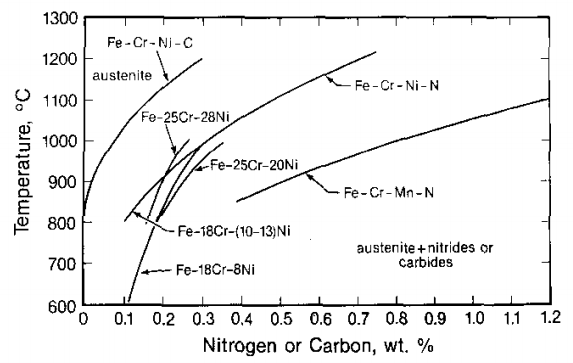
\includegraphics[width=0.8\textwidth]{solubN}
	\label{fig:diagrN}
	\centering
	\fonte{Reed, 1989}
	\end{figure}
	
	A dissolução do nitrogênio na austenita ocorre para quantidades relevantes, sem que haja formação de precipitados, apenas em temperaturas elevadas, a partir de aproximadamente 1000°C, como visto na Figura ~\ref{fig:diagrN} e na Figura ~\ref{fig:diagramaN}.\par
	
	\begin{figure}[ht]
	\caption{Diagrama de Fases do Nitrogênio em uma liga AISI 316, as linhas cinzas são isóbaras para a pressão de N$_{2}$}
	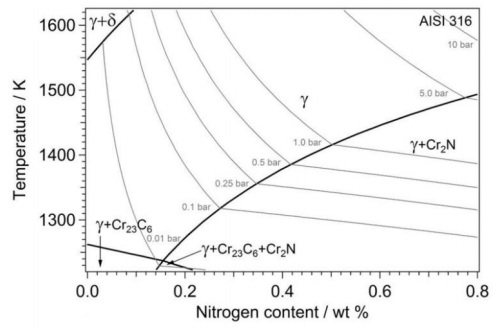
\includegraphics{diagramaN}
	\label{fig:diagramaN}
	\centering
	\fonte{SOMERS;CHRISITANSE;WINTHER, 2018}
	\end{figure}
	
	A formação de nitretos de cromo pode ser evitada pela adição de nitrogênio à temperaturas mais baixas, como mostra o diagrama TTT na Figura \ref{fig:TTTN}. Nessas temperaturas os átomos de nitrogênio se difundem pelos interstícios octaédricos do reticulado da austenita enquanto o cromo dissolve em uma taxa inferior por ser um substitucional e por isso apresenta um mecanismo de difusão mais lento. Dessa forma, é possível alcançar profundidades de difusão maiores sem que se formem nitretos.\par

	\begin{figure}[ht]
	\caption{Diagrama TTT esquemático}
	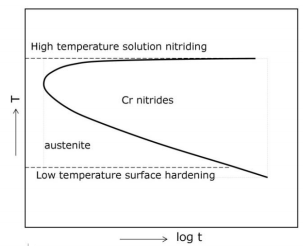
\includegraphics{TTTN}
	\label{fig:TTTN}
	\centering
    \fonte{SOMERS;CHRISITANSE;WINTHER, 2018}	
	\end{figure}
	
	A temperatura ideal para obtenção de um material com as propriedades desejadas deve ser inferior a 450°C para evitar a precipitação de CrN ~\cite{moskalioviene2011modeling}.
	Em soluções sólidas CFC, o cromo atrai o máximo de átomos de nitrogêno possível nos interstícios octaédricos vizinhos. Alguns dados experimentais mostram uma relação Cr:N entre 1:3 até 1:5 \cite{somers2018expanded}. Devido à grande afinidade entre esses dois elementos, é possível que ocorra uma solubidade metaestável de nitrogênio que supera o teor de nitrogênio que poderia estar na forma de nitretos ou dissolvido na matriz gerando uma solução sólida fortemente supersaturada.
	
\FloatBarrier

\subsection{Austenita Expandida}
	A austenita expandida ($\gamma_{N}$), também chamada de fase S,  é uma solução supersaturada de átomos intersiticiais (como nitrogênio e carbono) em austenita com concentrações de nitrogênio variando entre 9 a 20\%  ~\cite{williamson1994metastable} ou até 30\% ~\cite{moskalioviene2011modeling}. Ela é caracterizada por ser uma microsestrutura desenvolvida durante processos de endurecimento da superfície em temperaturas entre 350 e 400°C ~\cite{mandl2003nitrogen}. \par
	Como consequência dos interstícios supersaturados, essa fase apresenta uma expansão do reticulado cristalino, de até 11\% do parâmetro de rede e uma tensão residual de compressão associada elevada ~\cite{somers2018expanded}. Essa expansão pode facilitar a transferência de átomos de nitrogênio de um interstício octaédrico para um tetraédrico do reticulado CFC. Dessa forma, a energia de ativação para a difusão do nitrogênio é reduziada. Por outro lado, o aumento do teor de nitrogênio aumenta a ocupância dos interstícios, reduzindo a probabilidade do átomo em estado ativado conseguir mudar de uma posição para outra, o que reduz sua difusão \cite{christiansen2008nitrogen}. \par
	As propriedades da austenita expandida que a torna interessante economicamente são a elevada dureza, de até 15 GPa ~\cite{mandl2003nitrogen} e a redução da taxa de desgaste em 5 ordens de grandeza.


\section{Modelos}
	Os estudos do transporte de nitrogênio em aços austeníticos com formação de camadas superficiais constataram que o perfil de concentração dessa espécie não é consistente
	 com o perfil obtido pela resolução clássica da 2$^a$ Lei de Fick que considera o coeficiente de difusão independente da concentração para um sólido semi-infinito e concentração na superfície constante, como visto na seção \autoref{sec:difusao}. Na realidade, o perfil obtido é caracterizado por um platô seguido de uma queda brusca da concentração de nitrogênio \cite{parascandola2000nitrogen}. \par
	Na literatura encontram-se alguns modelos matemáticos que estudam a difusão do nitrogênio nos aços austeníticos, cada qual considerando um mecanismo predominante, um processo de nitretação e condições de contorno próprias. Os modelos podem ser dividos em algumas categorias, são elas: modelos que consideram um mecanismo de \textit{trapping-detrapping} dos átomos de nitrogênio perante o cromo ~\cite{parascandola2000nitrogen, moller2001surface, moskalioviene2011modeling}, modelos que consideram difusão com coeficiente de difusão dependente da concentração ~\cite{mandl2002concentration, mandl2003nitrogen}, aqueles que levam em consideração que a difusão é influênciada por tensões \cite{galdikas2010stress} e outros que combinam dois ou mais desses fatores ~\cite{christiansen2008nitrogen, moskalioviene2012stress}. Um resumo dos modelos analisados está listado na \autoref{tab:resumoModelos}.\par
	Outros fatores que influenciam na difusão do nitrogênio em aços e podem alterar os resultados no modelamento são o tratamento superficial anterior à nitretação \cite{baranowska2010importance}, o método utilizado nos experimentos em que se obteve um perfil para a concentração de nitrogênio ~\cite{moskalioviene2011modeling}, a orientação cristalina ~\cite{moskalioviene2011modeling}, no caso de nitretação a plasma:  alterações da superfície, tensões de compressão e rotação do reticulado  ~\cite{moskalioviene2011modeling}, camada superficial de óxido e segregação e dessegregação de elementos de liga próximos da superfície ~\cite{mandl2002concentration}.
	
\begin{table}[]
\centering
\setlength{\doublerulesep}{\arrayrulewidth}
{\def\arraystretch{2}\tabcolsep=10pt
\caption{Resumo dos Modelos Analisados}
\resizebox{\textwidth}{!}{%
\begin{tabular}{c C{3cm} C{3cm} C{3cm} C{3cm} C{3cm}}
\hline\hline
Trabalho & Método de Nitretação & Coeficiente de Difusão dependente da Concentração & Tensões & Trapping-Detrapping & Seção \\\hline
\cite{parascandola2000nitrogen} & Plasma (400°C) &  &  & X & \autoref{sec:trap-detrap} \\
\cite{moskalioviene2011modeling} & Plasma (400°C) &  &  & X & \autoref{sec:trap-detrap} \\
\cite{moller2001surface} & Implantação Iônica (400°C) &  &  & X & \autoref{sec:trap-detrap} \\
\cite{mandl2003nitrogen} & \begin{tabular}[C{3cm}]{@{}C{3cm}@{}}Implantação Iônica (380°C e 400°C)\\Implantação Iônica de Baixa Energia (400°C)\end{tabular} & X &  &  & \autoref{sec:concdep} \\
\cite{galdikas2010stress} & Plasma (400°C) &  & X &  & \autoref{sec:tensao} \\ 
\cite{christiansen2008nitrogen} & Gás (445°C) & X &  & X & \autoref{sec:comb-depc-td} \\
\cite{galdikas2011modeling} & Plasma (400°C) & X & X &  & \autoref{sec:comb-depc-stress} \\
\hline\hline
\end{tabular}
\label{tab:resumoModelos}
}
}
\end{table}


\subsection{Modelos \textit{trapping-detrapping}}
\label{sec:trap-detrap}
	O mecanismo de trapping-detrapping considera que os átomos de Cr aprisionam átomos de N devido à alta afinidade entre ambos, criando camadas superficiais enriquecidas em N com concentrações próximas ou maiores que as de Cr ~\cite{parascandola2000nitrogen}. Segundo esse modelo, quando todos os átomos de cromo já estão associados à átomos de nitrogênio, os novos átomos que difundem pela superfície difundem rapidamente pela camada formada até a região aonde os átomos de cromo ainda não estão saturados de nitrogênio.  \par
	No modelo de ~\cite{parascandola2000nitrogen}, assumiu-se que a difusão de N em aços inoxidáveis austenítios ocorria por meio da influência de regiões de aprisionamnto representados por átomos de cromo na matriz austenítica estacionária formada por elementos substitucionais (ou seja, a difusão desses elementos não é considerada, o que se justifica pela baixa distância de difusão do Cr estimada e pela ausência de precipitação de CrN a 400°C). Além disso, considerou-se que o nitrogênio é aprsionado em interstícios da solução, sendo que cada região de aprisionamento pode deter um átomo desse elemento. Destaca-se que o fenômeno em questão segue cinética de primeira ordem. O fato de se considerar o desaprisionamento (\textit{detrapping}) possui como objetivo obter uma previsão mais quantitativa do transporte. \par
	Os autores ~\cite{moller2001surface} analisam o caso aonde o processo de nitretação é a implantação iônica à plasma, que apresenta íons com energia entre 0-10keV com alta capacidade de penetração da superfície. No estudo realizado para esse modelo constatou-se a importância do \textit{sputtering} na nitretação dos aços inoxidáves, uma vez que reduz a camada passiva de óxido que atua como uma barreira para o nitrogênio sendo implantado. Busca-se então relacionar o \textit{sputtering} com a cinética da nitretação e conclui-se que a nitretação com íons energéticos apresenta uma desvantagem perante a nitretação à plasma pois limita-se a espessura máxima nitretada devido ao \textit{sputtering}. \par
	O modelamento desenvolvido por ~\cite{moskalioviene2011modeling} considerou o mecanismo de \textit{trapping-detrapping} em aços inoxidáveis austeníticos policristalinos que foram tratados por nitretação a plasma com temperaturas próximas de 400°C, buscando considerar a anisotropia da difusão do nitrogênio. Para isso utilizaram-se diferentes coeficientes de difusão para diferentes orientações cristalográficas. Algumas considerações feitas nesse modelo são: o nitrogênio pode estar localizado em uma região na qual pode difundir ou em uma região de aprisionamento na qual não ocorre sua difusão, existe apenas um tipo de aprisionamento, a concentração de pontos de aprisionamento é constante no espaço e tempo, cada sítio pode aprisionar um único átomo, a energia de desaprisionamento é independente da fração de pontos potenciais ocupados, existe equilíbrio local entre nitrogênio em regiões livres e em regiões de aprisionamento e o aprisionamento e desaprisionamento são controlados por difusão e seguem cinética de primeira ordem.\par
	Críticas aos modelos que consideram o fenômeno de \textit{trapping-detrapping} afirmam que não é possível relacionar a mudança de comportamento no transporte de nitrogênio com o teor de cromo, visto que apesar de alguns experimentos mostrarem uma transição para concentrações de nitrogênio coincidentes com as de cromo, em outros a transição correspondia à teores de nitrogênio inferiores à de cromo e visto que a magnitude da energia de interação entre Cr-C é significamente menor que a do Cr-N, assumir que esse mecanismo atua para ambos átomos deve ser questionada ~\cite{mandl2002concentration}.
	
\subsection{Modelos para coeficiente de difusão dependente da concentração}
\label{sec:concdep}
	Ao desenvolver o modelo que considera um coeficiente de difusão do nitrogênio em aço inoxidável austenítico, ~\cite{mandl2003nitrogen} utilizou diferentes ligas e parâmetros experimentais com o objetivo de correlacionar a difusividade com a composição da liga de forma a prever o comportamento dos aços quando nitretados. As simplificações adotadas foram que a concentração de N na superfície era constante e apenas o nitrogênio é móvel em uma matriz estacionária (não há difusão de outros componentes).\par
	Os diferentes parâmetros adotados foram:
	\begin{itemize}
	 \item Para o aço X6CrNiMoTi17.12.2—DIN 1.4571/AISI 316Ti - de componiçaõ 0.06 p.\% C, 17 p.\% Cr, 12 p.\% Ni, 2 p.\% Mo, 0.5 p.\% Ti:
		\begin{itemize}
		 \item Tratamento por implantação iônica à plasma a 380°C por 4 horas com pulsos de 5$\mu$s a 40kV
		\end{itemize}
	 \item Para o aço X5CrNi18.10 (DIN 1.4301), com 18 p.\% Cr (sempre a 400°C):
		\begin{itemize}
		 \item Implantação iônica de baixa energia com 1keV e corrente de 0,5 mA/cm$^2$
		 \item Implantação iônica à plasma por 3 horas com pulsos de 100$\mu$s a 40 kV
		\end{itemize} 
	\end{itemize}
	Possíveis fontes de erro para esse modelo são a expansão do reticulado e a errosão da superfície causada pelo processo de \textit{sputtering}.
	Analisando o mecanismo de difusão do ponto de vista macroscópico, infere-se no artigo que o perfil de nitrogênio observado corresponde à difusão em duas fases distintas: a difusão na superfície corresponderia à difusão do nitrogênio na austenita expandida e aquela mais distante da superfície seria a difusão na austenita.\par

\subsection{Difusão induzida por Tensão}
\label{sec:tensao}
	Para construção desse modelo, levou-se em consideração que a expansão do reticulado na formação de austenita expandida promove tensões induzidas pelo gradiente de concentração do nitrogênio e que influencia na sua difusão. Tensão é um dos fatores que determinam o potencial químico de componentes de um sistema sólido \cite{galdikas2010stress}. \par
	 A força motriz do transporte de nitrogênio em aço está associado ao gradiente de potenical químico, que pode ser associado ao fluxo de difusão. Para utilizar essa informação, considerou-se que não há gradiente de temperatura, a atividade do nitrogênio na matriz de aço é igual a 1 (solução ideal) e que o transporte ocorre em uma dimensão. \par
	 O modelo se limita a estudar a distribuição de nitrogênio em aços inoxidáveis austeníticos para temperaturas inferiores à formação de nitretos de cromo (~400°C), aonde o  teor de nitrogênio na superfície não deve ultrapassar 35 at.\% dado que a partir desse valor podem precipitar nitretos e não pode ser aplicado para casos de correntes de alta densidade devido aos efeitos de \textit{sputtering} e surgimento de defeitos que não são previstos no trabalho em questão.
	 Considerou-se que o coeficiente de difusão não depende da concentração ou da profundidade e para definir o seu valor foram testados diferentes valores até encontrar o que apresentava melhor correlação aos dados experimentais.
	 
\subsection{Modelos que combinam fatores}
\subsubsection{Coeficiente de Difusão dependente da Concentração + \textit{trapping}}
\label{sec:comb-depc-td}
	Nesse modelo, elaborado por \cite{christiansen2008nitrogen}, a difusão do nitrogênio é abordada considerando que o coeficiente de difusão é dependente da concentração do átomo  e considera-se relevante para a construção do modelo a ordenação a curta distância entre o nitrogênio e o cromo (mecanismo de \textit{trapping} dos átomos de N pelos de Cr). Para isso o coeficiente de difusão foi aproximado por uma série de coeficientes efetivos em diferentes faixas de composição e posteriormente foi utilizado o método de Boltzmann-Matano pra obter a solução da equação com depedência da concentração. Esse modelo foi baseado naquele apresentado por \cite{sun1997numerical} para a difusão do nitrogênio em ligas de ferrita.\par
	O efeito do \textit{trapping} foi modelado considerando que a constante termodinâmica de solubilidade é dada pelo produto das composiçoes de nitrogênio e cromo, acima da qual ocore aprisionamento do nitrogênio pelo cromo.
	
	Nesse modelo foi considerado nitretação à gás (utilizando misturas de NH$_3$/H$_2$) sob o pretexto de que esse método permite um controle do potencial químico do nitrogênio através da fase gasosa, enquanto no tratamento à plasma o potencial depende também de fatores associados ao plasma e à propriedades relacionadas ao substrato catódico. Aconselha-se evitar o uso de plasma na análise do coeficiente de difusão pois a aceleração na implantanção de íons pode promover o surgimento de defeitos que afetam o transporte.\par
	Assumiu-se que na interface entre as fases gasosa e sólida há equilíbrio de composição, apesar de dados experimentais apontarem que a composição na superfície é menor que no caso em que há equilíbrio. Quando considerando uma concentração superficial constante, esta corresponde a concentração total devido ao aprisionamento, que aumenta a concentração total. Isto significa que quando o produto de solubilidade muda, a concentração de nitrogênio na superfície também muda para esse caso. Outras hipóteses consideradas são que não há precipitação de nitretos, dado que esse é o pretexto da metaestabilidade da austenita expandida em nitretação a baixas temperaturas e a difusão ocorre em um sistema com uma única fase.\par
	O artigo ainda aponta uma possível influência das tensões residuais de compressão da austenita expandida que pode influenciar no mecanismo de difusão e constata que a determinação do coeficiente de difusão utilizando o método de Boltzmann-Matano resulta em valores não condizentes com dados reais possivelmente dado a omissão do mecanismo de aprisionamento.
	
\subsubsection{Coeficiente de Difusão dependente da Concentração + Tensão}
\label{sec:comb-depc-stress}
	Complementando o modelo criado para difusão dependente da tensão \cite{galdikas2010stress}, adicionou-se a dependênia da concentração no coeficiente de difusão de acordo com a realação de Einstein-Smoluchowski D(C$_N$)=f(1/C$_N$) \cite{moskalioviene2012stress} e assumiu-se que o teor de nitrogênio aumenta com o tempo de tratamento, ou seja C$_N\sim$ (t$^b$), logo D $\sim$ (1/t$^b$) com b $\approx$ 1.
	As condições dos experimentos de nitretação à plasma utilizados para comparação com os daods calculados - que são também as condições consideradas para os cálculos - são: 
	\begin{itemize}
	 \item Composição do gás: 60\% N$_2$ + 40\%H$_2$
	 \item Pressão de trabalho de 7.5 Pa e amplificador de potência de 700 W
	 \item Temperatura do substrato de 400°C
	 \item Duração da nitretação de 1h, 3h e 8h
  	 \item Energia dos ions inferior à 15 eV (que é menor que o limite de \textit{sputtering} para muitos materiais)
	\end{itemize}
	

\chapter{Materiais e Métodos}
\section{Desenvolvimento}
Primeiramente foi simulada a solução clássica da Segunda Lei de Fick com coeficiente de difusão constante e concentração de átomos na superfície constante (Seções \ref{sec:sol-numerica-2alei}/\ref{sec:modelo11}). Em seguida foi feito um modelo considerando a variação da concentração de átomos na superfície (Seções \ref{sec:sol-numerica-2alei2}/\ref{sec:modelo12}). Posteriormente o modelo foi incrementado para melhor satisfazer a realidade da difusão do nitrogênio utilizando a teoria dos sítios de \textit{trapping-detrapping}, considerando concentração superficial constante (Seções \ref{sec:my-trapdetrap}/\ref{sec:modelo21}) e variável (Seções \ref{sec:trap-detrap-gas-cc}/\ref{sec:trap-detrap-plasma-cc}/\ref{sec:modelo22}/\ref{sec:modelo23}).
O código elaborado para o trabalho foi feito em python e pode ser observado nos anexos.

\section{Métodos Numéricos e Algoritmos}

\subsection{Método das Diferenças Finitas}
\label{sec:dif-fin}
\par Uma forma de encontrar a solução de equações diferenciais é pelo método das diferenças finitas. A ideia fundamental desse método é aproximar a derivada de uma função ao redor de um dado ponto utilizando valores desta função em pontos vizinhos, criando uma malha de nós sobre o domínio da função.
\par Considerando um problema de equações diferenciais com condições de Dirichlet (onde são conhecidos os valores nas extremidadades do domínio) representada pelo sistema $(S)$, podemos discretizar o intervalo [a, b] no pontos $x_i = a + ih$ para $i \in [0, n+1]$, sendo $h = \dfrac{b-a}{n+1}$, a distância entre os nós.

\begin{center}
	\begin{math}
		(S)
		\left\{
    		\begin{array}{l}
      			-u'' + p(x)u + q(x)u = g(x) \\
				u(a) = \alpha\\
				u(b) = \beta      			
    		\end{array}
    		\begin{array}{l}
      		\qquad \\
			\qquad \\
			\qquad	   
    		\end{array}
    		\begin{array}{l}
      			x \in [a, b] \\
				p, q, g \in C^0([a, b])\\
				q \geq 0 \ em \ [a, b]
    		\end{array}
		\right.
	\end{math}
\end{center} 

\par Seja $u_i$ o valor aproximado de $u(x_i)$ que deseja-se calcular e $U = (u_1, ..., u_n)^T$, $u_0 = \alpha$ e $u_{n+1} = \beta$. Aproxima-se $u''(x_i)$ e $u'(x_i)$ utilizando a série de Taylor de $u$ em torno de $x_i$.
\par A série de Taylor é a representação de uma função na forma de uma soma infinita cujos termos são calculados pelas derivadas da função em um único ponto.
A eq.(\ref{eq:taylor}) é a série de Taylor da funçao $f(x)$ em torno de $x_i$.

\begin{equation} \label{eq:taylor}
f(x_i) = \sum_{n=0}^\infty \dfrac{f^{(n)}(x_i)}{n!}(x-x_i)^n = f(x_i) + \dfrac{f'(x_i)(x-x_i)}{1!} + \dfrac{f''(x_i)(x-x_i)^2}{2!} + ... \;.
\end{equation}

Pode-se escrever a série de Taylor de $u$ em torno de $x_i$ como visto na eq.(\ref{eq:taylor-u}).

\begin{equation} \label{eq:taylor-u}
u(x) = u(x_i) + u'(x_i)(x-x_i) + \dfrac{u''(x_i)}{2!}(x-x_i)^2 + ...  \;.
\end{equation}

As expansões de Taylor para $u$ em torno e $x_i$, para $x=x_{i-1}$ e $x=x_{i+1}$ estão descritas nas equações eq.(\ref{eq:taylor-u-1}) e eq.(\ref{eq:taylor-u+1}), respectivamente.

\begin{equation} \label{eq:taylor-u-1}
u(x_{i-1}) = u(x_i-h) = u(x_i) - hu'(x_i) + \dfrac{h^2u''(x_i)}{2!} - \dfrac{h^3 u^{(3)}(x_i)}{3!} + O(h^4) \;.
\end{equation}


\begin{equation} \label{eq:taylor-u+1}
u(x_{i+1}) = u(x_i+h) = u(x_i) + hu'(x_i) + \dfrac{h^2u''(x_i)}{2!} + \dfrac{h^3 u^{(3)}(x_i)}{3!} + O(h^4) \;.
\end{equation}

Subtraindo a eq.(\ref{eq:taylor-u-1}) da eq.(\ref{eq:taylor-u+1}), obtém-se:

\begin{equation} \label{eq:u-linha}
\dfrac{u(x_{i+1}) - u(x_{i-1})}{2h} = u'(x_i) + O(h^2) \;.
\end{equation}

E somando as mesmas equações:

\begin{equation} \label{eq:u-linha-linha}
\dfrac{u(x_{i+1}) -2u(x_i) + u(x_{i-1)}}{h^2} = u''(x_i) + O(h^2) \;.
\end{equation}

Subsitituindo as equações eq.(\ref{eq:u-linha}) e eq.(\ref{eq:u-linha-linha}) em $(S)$, obtém-se:

\begin{equation} 
\dfrac{u(x_{i+1}) -2u(x_i) + u(x_{i-1})}{h^2} + p(x_i)\dfrac{u(x_{i+1}) - u(x_{i-1})}{2h}  + q(x_i)u(x_i) - g(x_i) = e_i \;.
\end{equation}

para todo $i=1, ..., n$ com $e_i = O(h^2)$ chamado de erro de truncamento.
 
\par Logo, utilizando a notação $p_i = p(x_i)$, $q_i = q(x_i)$, $g_i = g(x_i)$, o probelma $(S)$ pode ser reescrito como:

\begin{center}
	\begin{math}
		(S)
		\left\{
    		\begin{array}{l}
      			\dfrac{-u_{i+1}+ 2u_i - u_{i-1}}{h^2} + p_i\dfrac{u_{i+1} - u_{i-1}}{2h}  + q_i u_i - g_i = 0 \\
				u_0 = \alpha\\
				u_{n+1} = \beta      			
    		\end{array}
    		\begin{array}{l}
      		\qquad \\
			\qquad \\
			\qquad	   
    		\end{array}
    		\begin{array}{l}
      			i = 1, ... , n \;.
    		\end{array}
		\right.
	\end{math}
\end{center} 

O problema dado por $(S)$ consiste de um sistema de $n$ equações lineares com $n$ incógnitas que pode ser escrito de forma matricial: \cmrtext{AU=B}, com \cmrtext{A=$M_n$($\mathbb{R}$)}, \cmrtext{U=($u_1, u_2, ... , u_n)^T$} e \cmrtext{B $\in \mathbb{R}^n$}.


\begin{equation*}
	\cmrtext{A} =
	\begin{bmatrix}
		2+h^2q_1 & -1+\dfrac{h}{2}p_1 & \ldots  & \ldots & \ldots & 0 \\
		-1+\dfrac{h}{2}p_2 & 2+h^2q_2 & -1+\dfrac{h}{2}p_2 &  & & \vdots\\
		\vdots &\ddots&\ddots&\ddots&& \vdots \\
		\vdots &&\ddots&\ddots&\ddots& \vdots \\
		\vdots & & & \ddots & \ddots & -1+\dfrac{h}{2}p_{n-1} \\
		0 & \ldots & \ldots & \ldots & -1+\dfrac{h}{2}p_n & 2+h^2q_n	
	\end{bmatrix}
\end{equation*}

\begin{equation*}
	\cmrtext{U} =
	\begin{bmatrix}
		u_1 \\
		u_2 \\
		\vdots \\
		\vdots \\
		\vdots \\
		u_{n-1} \\
		u_n
	\end{bmatrix}
	\qquad
	\cmrtext{B} =
	\begin{bmatrix}
		h^2g_1 + \alpha(1+\dfrac{h}{2}p_1) \\
		h^2g_2 \\
		\vdots \\
		\vdots \\
		\vdots \\
		h^2g_{n-1} \\
		h^2g_{n} + \beta(1+\dfrac{h}{2}p_n)
	\end{bmatrix}
\end{equation*}

Esse sistema de equações pode ser resolvido utilizando o algoritmo da matriz tridiagonal (algoritmo de Thomas), apresentado na seção \ref{sec:algo-thomas}.

O método das diferenças finitas amplifica erros causados pelos truncamentos e arredondamentos a cada passo de tempo. Para identificar instabilidade escreve-se a equação para um nó de forma que ao seu lado esquerdo esteja somente a incógnita para a variável dependente daquele nó, se algum coeficiente das variáveis dependentes ao seu lado direito for negativo, é instável. O método explícito é semi-instável, o método implícito é incodicionalmente estável como será demonstrado na seção \ref{sec:sol-numerica-2alei} 

\subsection{Algoritmo de Thomas}	
\label{sec:algo-thomas}
O Algoritmo de Thomas é um algoritmo de resolução de sistemas de equações represetados por uma matriz tridiagonal e é uma simplificação da Eliminação Gaussiana ($\frac{2}{3}O(n^3)$), com custo $O(n)$.

Um sistema de equações cujo conjunto de equações possa ser representado pela eq.(\ref{eq:thomas-sistema1}), também pode ser escrita matricialmente, na forma de matriz tridiagonal.
\begin{equation}
\label{eq:thomas-sistema1}
a_i x_{i-1} + b_i x_i + c_i x_{i+1} = d_i \qquad i = 1, ..., n
\end{equation}

\begin{equation*}
	\begin{bmatrix}
		b_1 & c_1 &         &        & 0\\
		a_2 & b_2 &   c_2   &        & \\
		    & a_3 &   b_3   & \ddots & \\
		    &     &  \ddots & \ddots & c_{n-1} \\
	     0  &     &         &  a_n   & b_n 
	\end{bmatrix}
	\begin{bmatrix}
		x_1 \\
		x_2 \\
		x_3 \\
		\vdots \\
		x_n
	\end{bmatrix}
	=\begin{bmatrix}
		d_1 \\
		d_2 \\
		d_3 \\
		\vdots \\
		d_n
	\end{bmatrix}
\end{equation*}

Com algumas operações chega-se ao algoritmo em si - seja $L_i$ a linha $i$ do sistema:

\begin{equation*}
	L_1' = L_1 \divisionsymbol b_1 \Rightarrow
	\begin{bmatrix}
		1 & \dfrac{c_1}{b_1} &         &        & 0\\
		a_2 & b_2 &   c_2   &        & \\
		    & a_3 &   b_3   & \ddots & \\
		    &     &  \ddots & \ddots & c_{n-1} \\
	     0  &     &         &  a_n   & b_n 
	\end{bmatrix}
	\begin{bmatrix}
		x_1 \\
		x_2 \\
		x_3 \\
		\vdots \\
		x_n
	\end{bmatrix}
	=\begin{bmatrix}
		\dfrac{d_1}{b_1} \\
		d_2 \\
		d_3 \\
		\vdots \\
		d_n
	\end{bmatrix}
\end{equation*}

\begin{equation*}
	L_2' = L_2 - a_2L_1'  \Rightarrow
	\begin{bmatrix}
		1 & \dfrac{c_1}{b_1} &         &        & 0\\
		0 & b_2 - a_2\dfrac{c_1}{b_1} &   c_2   &        & \\
		    & a_3 &   b_3   & \ddots & \\
		    &     &  \ddots & \ddots & c_{n-1} \\
	     0  &     &         &  a_n   & b_n 
	\end{bmatrix}
	\begin{bmatrix}
		x_1 \\
		x_2 \\
		x_3 \\
		\vdots \\
		x_n
	\end{bmatrix}
	=\begin{bmatrix}
		\dfrac{d_1}{b_1} \\
		d_2 - a_2\dfrac{d_1}{b_1}\\
		d_3 \\
		\vdots \\
		d_n
	\end{bmatrix}
\end{equation*}

Seja $c_1' = \dfrac{c1}{b1}$ e $d_1' = \dfrac{d1}{b1}$:
\begin{equation*}
	L_2'' = L_2'\divisionsymbol (b_2-a_2c_1')  \Rightarrow
	\begin{bmatrix}
		1 & c_1' &         &        & 0\\
		0 & 1 &   \dfrac{c_2}{b_2-a_2c_1'}   &        & \\
		    & a_3 &   b_3   & \ddots & \\
		    &     &  \ddots & \ddots & c_{n-1} \\
	     0  &     &         &  a_n   & b_n 
	\end{bmatrix}
	\begin{bmatrix}
		x_1 \\
		x_2 \\
		x_3 \\
		\vdots \\
		x_n
	\end{bmatrix}
	=\begin{bmatrix}
		d_1' \\
		\dfrac{d_2 - a_2d_1'}{b_2-a_2c_1'}\\
		d_3 \\
		\vdots \\
		d_n
	\end{bmatrix}
\end{equation*}

De forma análoga para as outras linhas, chega-se que:

\begin{center}
	\begin{math}
		c_i' = 
		\left\{
    		\begin{array}{l}
      			\dfrac{c_i}{b_i}  \\
				\dfrac{c_i}{b_i - a_i c_{i-1}'}
			\end{array}
    		\begin{array}{l}
      		\qquad \\
			\qquad \\
			\qquad	   
    		\end{array}
    		\begin{array}{l}
    			i = 1 \\
      			i = 2, ... , n-1
    		\end{array}
		\right.	
	\end{math}
\end{center} 
\begin{center}
	\begin{math}
		d_i' = 
		\left\{
    		\begin{array}{l}
      			\dfrac{d_i}{b_i}  \\
				\dfrac{d_i - a_i d_{i-1}'}{b_i - a_i c_{i-1}'}
			\end{array}
    		\begin{array}{l}
      			\qquad \\
				\qquad \\
				\qquad	   
    		\end{array}
    		\begin{array}{l}
    			i = 1 \\
      			i = 2, ... , n
    		\end{array}
		\right.
	\end{math}
\end{center} 

Dessa forma, a solução para o sistema de equações encontrand $x_n$, $x_{n-1}$, $x_{n-2}$, ..., até $x_1$ utilizando:

\begin{gather*}
	x_n = d_n' \\
	x_i = d_i' - c_i' x_{i+1} \ para \ i = 1, ..., n-1
\end{gather*}

\section{Solução Numérica da Segunda Lei de Fick}
\subsection{Composição Superficial Constante}
\label{sec:sol-numerica-2alei}
Recordando a Segunda Lei de Fick mencionada na seção \ref{sec:difusao}, estuda-se uma solução numérica para a equação diferencial \ref{eq:2alei-num}.

\begin{equation}
\label{eq:2alei-num}
\pdv{C(x,t)}{t} = D(C)\pdv[2]{C(x,t)}{x}
\end{equation}

Para essa solução, considera-se o coeficiente de difusão constante (independente da concentração, temos D(C) = D. Utilizando o método das diferenças finitas apresentado na seção \ref{sec:dif-fin}, a discretização do espaço será dada por um espaçamento {$\Delta x$}, e representa-se por $i$ o i-ésimo nó do eixo x. Para o passo do tempo, utilizou-se um passo {$\Delta t$}, e $j$ nota o j-ésimo instante de tempo. Assim, tem-se a representação discretizada da eq.\ref{eq:2alei-num} dada pela eq.\ref{eq:2alei-discr}. Destaca-se que foi utilizado o método implícito das diferenças finitas para a realização do trabalho.

\begin{equation}
\label{eq:2alei-discr}
\dfrac{C_i^{j+1} - C_i^j}{\Delta t} = D\dfrac{C_{i+1}^{j+1} - 2C_i^{j+1} + C_{i-1}^{j+1}}{(\Delta x)^2}
\end{equation}

\myworries{colocar o grafico mostrando os nós}


As condições de contorno adotadas serão as mesmas apresentadas na seção \ref{sec:difusao}, isto é, a concentração inicial de N no interior do material é nula e a concentração na superfície se mantém constante ao longo do tempo. Essas condições podem ser descritas da seguinte forma:

\begin{gather*}
		\mathrm{Condição\ Inicial: }\ C(x, t=0) = c_i^0 = 0 \qquad i \in [0;\ n+1] \\
		\mathrm{Condições\ de\ Contorno:}\ 
		\left\{
    		\begin{array}{l}
      			C(x=0, t>0) = C_0^j = C_s  \\
				C(x\rightarrow\infty, t>0) = C_{n+1}^j = 0 
			\end{array}
    		\begin{array}{l}
      		\qquad \\
			\qquad \\	   
    		\end{array}
    		\begin{array}{l}
    			j \in [0,\ T] 
    		\end{array}
		\right.	
\end{gather*}


A eq.(\ref{eq:2alei-discr}) pode ser reescrita como:

\begin{equation}
\label{eq:antesFo}
C_i^{j+1} - \frac{D\Delta t}{(\Delta x)^2} (C_{i+1}^{j+1} - 2C_i^{j+1} + C_{i-1}^{j+1}) = C_i^j
\end{equation}

A relação $\dfrac{D\Delta t}{(\Delta x)^2}$ é um número adimensional chamado de número de Fourier. Seja $Fo = \dfrac{D\Delta t}{(\Delta x)^2} $. Reescrevemos a eq.\ref{eq:antesFo} subsitindo com $Fo$, isolando a incógnita ao lado esquerdo:

\begin{gather*}
\label{eq:depoisFo}
- FoC_{i+1}^{j+1} + (1+2Fo)C_i^{j+1} - FoC_{i-1}^{j+1} = C_i^j \\
C_i^{j+1} = \dfrac{1}{(1+2Fo)}C_i^j + \dfrac{Fo}{(1+2Fo)}C_{i-1}^{j+1} + \dfrac{Fo}{(1+2Fo)}C_{i+1}^{j+1}
\end{gather*}

Segundo o critério de estabilidade mencionado na seção \ref{sec:dif-fin}, como $Fo>0$, o esquema implícito é sempre estável.

Agora desenvolve-se o sistema de equações para resolver o problema diferencial.

\begin{equation*}
\label{eq:depoisFo}
\begin{matrix}
i = 1: \qquad -FoC_{0}^{j+1} + (1+2Fo)C_1^{j+1} - FoC_{2}^{j+1} - C_1^j & = & 0\\
(1+2Fo)C_1^{j+1} - FoC_{2}^{j+1}& = & FoC_{s}^{j+1}  + C_1^j \\ 
\\
i = 2: \qquad -FoC_{1}^{j+1} + (1+2Fo)C_2^{j+1} - FoC_{3}^{j+1} - C_2^j & = & 0\\
(1+2Fo)C_2^{j+1} - FoC_{3}^{j+1} - FoC_{1}^{j+1} & = & C_2^j \\ 
\vdots \\
i = n: \qquad -FoC_{n-1}^{j+1} + (1+2Fo)C_n^{j+1} - FoC_{n+1}^{j+1} - C_n^j & = & 0\\
(1+2Fo)C_n^{j+1} - FoC_{n-1}^{j+1} & = & C_n^j \\ 
\end{matrix}
\end{equation*}

Seja o sistema de equações dado por \cmrtext{AC$^{j+1}$ = B$^j$}, \cmrtext{A, C e B} podem ser definidos por:

\begin{equation*}
	\cmrtext{A} =
	\begin{bmatrix}
		(1+2Fo) & -Fo &         &        & 0\\
		-Fo & (1+2Fo) &  -Fo   &        & \\
		    & -Fo &   (1+2Fo)   & \ddots & \\
		    &     &  \ddots & \ddots & -Fo \\
	     0  &     &         &  -Fo   & (1+2Fo) 
	\end{bmatrix}
\end{equation*}
\begin{equation*}
	\cmrtext{C^{j+1}} =
	\begin{bmatrix}
		c_1^{j+1} \\
		c_2^{j+1} \\
		c_3^{j+1} \\
		\vdots \\
		c_n^{j+1}
	\end{bmatrix}
	\qquad
	\cmrtext{B^j} =	
	\begin{bmatrix}
		Fo\ c_s+c_1^j \\
		c_2^{j} \\
		c_3^{j} \\
		\vdots \\
		c_n^{j}
	\end{bmatrix}
\end{equation*}

\cmrtext{A} é uma matriz tridiagonal, \cmrtext{AC$^{j+1}$ = B$^j$} é um sistema de $n$ equações lineares com $n$ incógnitas. Logo, pode-se utilizar o algoritmo de Thomas visto na seção \ref{sec:algo-thomas} para solucionar o problema.

\subsection{Composição Superficial Variável}
\label{sec:sol-numerica-2alei2}
Para o caso de nitretação gasosa, segundo o artigo de \cite{christiansen2008nitrogen}, uma forma de simular a concentração na superfície é utilizando a relação dada pela equação \autoref{eq:cs-gas}. Na qual, t é o instante de tempo, $\beta$ determina a velocidade com que a concentração na superfície atinge a concentração em equilíbrio e $C_{\infty}$ é a concentração de equilíbrio para o gás e o aço.

\begin{equation}
\label{eq:cs-gas}
C_{s}(t) = C_{\infty}(1 - e^{\beta t})
\end{equation}

Sendo assim, basta substituir $C_s^{j+1} = C_{\infty}(1 - e^{\beta j\Delta t})$ no desenvolvimento realizado na seção \autoref{sec:modelo11}, de forma que o sistema apresentado (\cmrtext{AC$^{j+1}$ = B$^j$}) tenha uma equação para $c_0$:

\begin{equation*}
	\cmrtext{A} =
	\begin{bmatrix}
		  1 & 0 &         &        & 0\\
		-Fo & (1+2Fo) &  -Fo   &        & \\
		    & -Fo &   (1+2Fo)   & \ddots & \\
		    &     &  \ddots & \ddots & -Fo \\
	     0  &     &         &  -Fo   & (1+2Fo) 
	\end{bmatrix}
\end{equation*}
\begin{equation*}
	\cmrtext{C^{j+1}} =
	\begin{bmatrix}
		c_0^{j+1} \\
		c_1^{j+1} \\
		c_2^{j+1} \\
		\vdots \\
		c_n^{j+1}
	\end{bmatrix}
	\qquad
	\cmrtext{B^j} =	
	\begin{bmatrix}
		C_{\infty}(1 - e^{\beta j\Delta t}) \\
		c_1^j \\
		c_2^{j} \\
		\vdots \\
		c_n^{j}
	\end{bmatrix}
\end{equation*}



Para considerar a varição na concentração da superfície, pode-se utilizar um termo de adsorção na condição de contorno, como foi utilizado por \cite{galdikas2011modeling}, dado por $\dfrac{\alpha j}{qN_{superfície}}\left(H_0-C(0,t)\right)$, onde $j$ representa a densidade de corrente média do íon de nitrogênio, $\alpha$ é o coeficiente de adesão do nitrogênio nos componentes, $q$ é a carga elementar (equivalente a $1,602.10^{-19}C$), $N_{superfície}$ é a concentração de átomos na superfície (em átomos por $m^2$), $H_0$ é  concentração de átomos hospedeiros e $C(0,t)$ é a concentração de átomos de nitrogênio na superfície.

As equações da seção \ref{sec:sol-numerica-2alei} se mantêm as mesmas, exceto pelo contorno que define a superfície pela qual ocorre adsorção, que é descrito pela eq.\autoref{eq:2alei-num-plasma}

\begin{equation}
\label{eq:2alei-num-plasma}
\pdv{C(x,t)}{t} = D(C)\pdv[2]{C(x,t)}{x} + \dfrac{\alpha j}{qN_{superfície}}\left(H_0-C(0,t)\right)
\end{equation}

As condições iniciais e a condição de contorno para $x\rightarrow\infty$ não se alteram.

Discretizando a equação \autoref{eq:2alei-num-plasma}, utilizando $j_0 = \dfrac{j}{qN_{superfície}}$ obtêm-se:

\begin{gather*}
\dfrac{C_0^{j+1} - C_0^j}{\Delta t} = D\dfrac{C_{i+1}^{j+1} - C_{i}^{j+1}}{(\Delta x)^2} + \alpha j_0\left(H_0-C(0,t)\right) 
\end{gather*}

\begin{equation}
\label{eq:2alei-num-plasma-discr}
C_0^{j+1} = C_0^j - Fo(C_{1}^{j+1} - C_{0}^{j+1})+ \alpha j_0 \Delta t \left(H_0-C_{0}^{j+1}\right)  \qquad   j \in [0,\ T]
\end{equation}

Para resolver o probelma diferencial, desenvolve-se o sistema de equações:

\begin{equation*}
\label{eq:depoisFo}
\begin{matrix}
i = 0: \qquad (1- Fo + \alpha j_0 \Delta t)C_0^{j+1} + FoC_{1}^{j+1} & = & C_0^j + \alpha j_0 \Delta t H_0 \\
\\
i = 1: \qquad FoC_{0}^{j+1} - (1+2Fo)C_1^{j+1} + FoC_{2}^{j+1} + C_1^j & = & 0\\
(1+2Fo)C_1^{j+1} - FoC_{2}^{j+1} - FoC_{0}^{j+1} & = & C_1^j \\ 
\\
i = 2: \qquad FoC_{1}^{j+1} - (1+2Fo)C_2^{j+1} + FoC_{3}^{j+1} + C_2^j & = & 0\\
(1+2Fo)C_2^{j+1} - FoC_{3}^{j+1} - FoC_{1}^{j+1} & = & C_2^j \\ 
\vdots \\
i = n: \qquad FoC_{n-1}^{j+1} - (1+2Fo)C_n^{j+1} + FoC_{n+1}^{j+1} + C_n^j & = & 0\\
(1+2Fo)C_n^{j+1} - FoC_{n-1}^{j+1} & = & C_n^j \\
\end{matrix}
\end{equation*}

Analogamente ao que foi feito na seção \ref{sec:sol-numerica-2a-lei}, considerando o sistema de equações dado por \cmrtext{AC$^j+1$ = B$^j$}, \cmrtext{A, C e B} podem ser definidos por:

\begin{equation*}
	\cmrtext{A} =
	\begin{bmatrix}
		(1- Fo + \alpha j_0 \Delta t) & Fo &         &        & 0\\
		-Fo & (1+2Fo) &  -Fo   &        & \\
		    & -Fo &   (1+2Fo)   & \ddots & \\
		    &     &  \ddots & \ddots & -Fo \\
	     0  &     &         &  -Fo   & (1+2Fo) 
	\end{bmatrix}
\end{equation*}
\begin{equation*}
	\cmrtext{C^{j+1}} =
	\begin{bmatrix}
		c_0^{j+1} \\
		c_1^{j+1} \\
		c_2^{j+1} \\
		\vdots \\
		c_n^{j+1}
	\end{bmatrix}
	\qquad
	\cmrtext{B^j} =	
	\begin{bmatrix}
	c_0^j + \alpha j_0 \Delta t H_0 \\
		Fo\ c_s+c_1^j \\
		c_2^{j} \\
		\vdots \\
		c_n^{j}
	\end{bmatrix}
\end{equation*}

\cmrtext{A} é uma matriz tridiagonal, \cmrtext{AC$^{j+1}$ = B$^j$} é um sistema de $n$ equações lineares com $n$ incógnitas. Logo, também é possível utilizar o algoritmo de Thomas visto na seção \ref{sec:algo-thomas} para solucionar o problema.

Para o caso de nitretação gasosa ......



\section{Modelo de \textit{Trapping-Detrapping}}
\label{sec:my-trapdetrap}
Como descrito na seção \autoref{sec:trap-detrap}, o modelo de \textit{trapping-detrapping} considera que os átomos de Cromo em solução sólida nos aços agem como sítios de aprisionamento de Nitrogênio. Isso ocorre devido à alta afinidade ente os dois átomos.

Para considerar esse fenômeno foi adicionado um termo adicional à equação da Segunda Lei de Fick (eq.\autoref{eq:2alei-num}), $S(x)$ que permite considerar os efeitos do aprisionamento. Essa abordagem é uma adaptação do modelo criado em \cite{moskalioviene2011modeling}.

Nessa seção será utilizada a seguinte notação: $N_{dif}$ corresponde à concentração de nitrogênio disponível para difusão (não aprisionado), $N_{trap}$ será a concentração de nitrogênio no estado aprisionado e $N$ é a concentração total de nitrogênio em solução.

\begin{equation}
\label{eq:trap-detrap}
\pdv{N_{dif}(x,t)}{t} = D\pdv[2]{N_{dif}(x,t)}{x} - S(x,t)
\end{equation}

A equação \autoref{eq:trap-detrap}, juntamente com as equações \autoref{eq:trap-detrap2} e \autoref{eq:trap-detrap3} formam um conjunto de equações que descrevem o transporte de massa do nitrogênio considerando o mecanismo estudado.

\begin{equation}
\label{eq:trap-detrap2}
\pdv{N_{trap}(x,t)}{t} = S(x,t) = K\left[N_{dif}(x,t)\left(H_t-N_{trap}(x,t)\right) -N_0 N_{trap}(x,t)e^\dfrac{E_B}{k_BT}\right] 
\end{equation}

Segue o que representa cada termo da equação \autoref{eq:trap-detrap2}:

$K=4{\pi}R_tD$ : representa uma área (com raio $R_t$) de aprisionamento de um único sítio de aprisionamento

$D=D_0e^\dfrac{E_B}{k_BT}$
	$k_B$: constante de Boltzmann \myworries{(colocar o valor e a ref)}
	
	$T$: temperatura
	
\begin{equation}
\label{eq:trap-detrap3}
\pdv{N(x,t)}{t} = \pdv{N_{dif}(x,t)}{t} + \pdv{N_{trap}(x,t)}{t}
\end{equation}





\subsection{Discretização}
Para o coeficiente de difusão constante, a discretização das equações \autoref{eq:trap-detrap} e \autoref{eq:trap-detrap2} pelo método explícito segue:

Para a concentração de nitrogênio em solução sólida:
\begin{equation*}
\dfrac{{N_{dif}}_{i}^{j+1} - {N_{dif}}_{i}^{j}}{\Delta j} = D \dfrac{{N_{dif}}_{i+1}^{j} - 2{N_{dif}}_i^{j} + {N_{dif}}_{i-1}^{j}}{(\Delta i)^2} - S_i^j
\end{equation*} 

\begin{equation}
\label{eq:trap-detrap-discr2}
{N_{dif}}_{i}^{j+1} = {N_{dif}}_{i}^{j} + Fo({N_{dif}}_{i+1}^{j} - 2{N_{dif}}_i^{j} + {N_{dif}}_{i-1}^{j}) - {\Delta j} S_i^j
\end{equation} 


Para a concentração de nitrogênio aprisionado:
\begin{equation*}
S_i^j = \dfrac{{N_{trap}}_i^{j+1} - {N_{trap}}_{i}^{j}}{\Delta j} = k_t\left[{N_{dif}}_{i}^{j} \left(H_t-{N_{trap}}_{i}^{j}\right)\right] - k_d{N_{trap}}_i^{j}
\end{equation*}


\begin{equation}
\label{eq:trap-detrap2-discr2}
{N_{trap}}_i^{j+1} = {N_{trap}}_{i}^{j} + {\Delta j}\left[k_t\left({N_{dif}}_{i}^{j} \left(H_t-{N_{trap}}_{i}^{j}\right)\right) - k_d{N_{trap}}_i^{j}\right]
\end{equation}

\myworries{add algum comentario sobre as ccs}

Com as equações \autoref{eq:trap-detrap-discr2} e \autoref{eq:trap-detrap2-discr2} é possível resolver computacionalmente o problema.


\section{Parâmetros e Constantes}
\label{sec:params}


Os parâmetros utilizados estão explicitados na Tabela \ref{tab:resumoParametros}. Todos os valores de parâmetros que não são conhecidos da literatura foram retirados de \cite{moskalioviene2011modeling}.

\begin{table}[]
\centering
\setlength{\doublerulesep}{\arrayrulewidth}
{\def\arraystretch{2}\tabcolsep=10pt
\caption{Parâmetros}
\resizebox{\textwidth}{!}{%
\begin{tabular}{c c c C{4cm}}
\hline\hline
Parâmetro & Descrição & Valor & Obs \\\hline
$E_A$ & Energia de ativação de Difusão & $1,7622 10^{-19} J$  \\
$E_B$ & Energia de ativação de \textit{detrapping} & $4,48609 10^{-20} J$  \\\
$D_0$ & Fator pré-exponencial de difusão & $8,37 10^{-8} m^2/s$  \\
$H_0$  & Concentração de Átomos Hospedeiros& $H_0 = 4(1/R_t)^3 = 7,29 10^{28} m^{-3}$ & o fator 4 aparece pois existem 4 átomos hospedeiros por célula unitária \cite{peng2018numerical} \\
$H_t$  & Concentração de Sítios de Aprisionamento & $H_t = 0.18H_0 = 1,31 10^{-28}$ \\ 
$k_B$  & Constante de Boltzmann & $ 1,38064852 10^{-23} J/K$ \\ 
\hline\hline
\end{tabular}
\label{tab:resumoParametros}
}
}
\end{table}



\chapter{Resultados}
	Foram simulados dois modelos distintos - um dado pela Segunda Lei de Fick e outro dado pelo mecanismo de \textit{trapping-detrapping}, para três condições de contorno distintas: concentração superfícal constante, nitretaçao gasosa e nitretação à plasma.
	
	Com o objetivo de validar o modelo, foram utilizados dados experimentais obtidos de artigos de autores referenciados anteriormente. No caso da nitretação gasosa, foi disponibilizado pelo Dr Marcel Somers o resultado do experimento utilizado no artigo \cite{christiansen2008nitrogen} e para a nitretação à plasma foram retirados os dados do artigo \cite{moskalioviene2011modeling} utilizando o software WebPlotDigitizer.
	
	Para cada simulação, todas as entradas podem ser consultadas nas tabelas correspondentes encontradas no Anexo A.

\section{Modelo 1 - Segunda Lei de Fick}

\subsection{Concentração na superfície constante}
\label{sec:modelo11}
Para definir um valor para a concentração da superfície para implementação da solução clássica da Segunda Lei de Fick como descrito na Seção \autoref{sec:sol-numerica-2alei}, foi utilizado o artigo  \cite{christiansen2008nitrogen}, que possui o valor da ocupância de átomos de nitrogênio $y_N^{S}$ (mais especificamente a fração de interstícios octaédricos do reticulado cúbico de face centrada ocupada por nitrogênio) para o estado de equilíbrio, com $K_N=$2,49 $bar^{1/2}$ (valor para o qual os dados experimentais do artigo em questão mostravam-se mais próximos dos dados do modelo), para 445°C (718K). A variável $K_N=\dfrac{p_{NH_3}}{p_{H_2}^{3/2}}$ é o potencial de nitretação para uma mistura gasosa de NH$_3$/H$_2$.

A partir do valor de $y_N^{eq}$, para uma temperatura de 718K, é possível definir a concentração em $mols/m^3$ de nitrogênio utilizando a relação apresentada no apêndice A2 do artigo \cite{jespersen2016modelling}, dada pela equação\autoref{eq:oc-to-m3}.

\begin{equation} \label{eq:oc-to-m3}
	C = \dfrac{4}{N_A} \cdot y_N \cdot \dfrac{1}{V(y_N)}
\end{equation}

O fator 4 é o número de interstícios octaédricos de uma célula unitária CFC, $N_A$ é o número de Avogadro ($N_A = 6,0221409 \times 10^{23} (mol^{-1})$) e $V(y_N)$ é o volume da célula unitária (em $m^3$) para uma dada ocupância de nitrogênio.

A função $V(y_N)$ foi aproximada por uma função linear: 
\begin{gather*}
	V(y_N) = 2,8147 \times 10^{-29} \cdot y_N + 4,7134 \times 10^{-29}
\end{gather*}

Sendo assim, pode-se reescrever a equação \autoref{eq:oc-to-m3} como:

\begin{equation} \label{eq:oc-to-m3-full}
	C = \dfrac{4}{6,0221409 \times 10^{23}} \cdot \dfrac{y_N}{2,8147 \times 10^{-29} \cdot y_N + 4,7134 \times 10^{-29}}
\end{equation}

Dessa forma, para as condições especificadas acima, o valor de $y_N$ é 0,28 e a concentrção é 33.805 mol/m$^3$ (2,0358 $\times$ 10$^{28}$ m$^-3$).

\begin{table}[ht]
\centering
\setlength{\doublerulesep}{\arrayrulewidth}
{\def\arraystretch{2}\tabcolsep=10pt
\caption{Parâmetros para concentração na superfície constante}
\resizebox{\textwidth}{!}{
\begin{tabular}{c c c}
\hline\hline
Parâmetro & Descrição & Valor \\\hline

$C_{eq}$ & Concentração de equilíbrio entre gás e aço &  47.318,64 mol/m$^3$ (2,0358 $\times$ 10$^{28}$ m$^-3$)   \\
\hline\hline
\end{tabular}
\label{tab:parametros_csvar}
}
}
\end{table}

Os valores de $\Delta t$ e $\Delta x$ utilizados foram 0,01s e 0,1 $\mu m$. Para um tempo total de 22 horas e 20 $\mu m$ de profundidade, com temperatura igual a .



\begin{figure}[ht]
\centering
	\caption{Resultado simulação para concentração na superfície constante até 2 horas}
	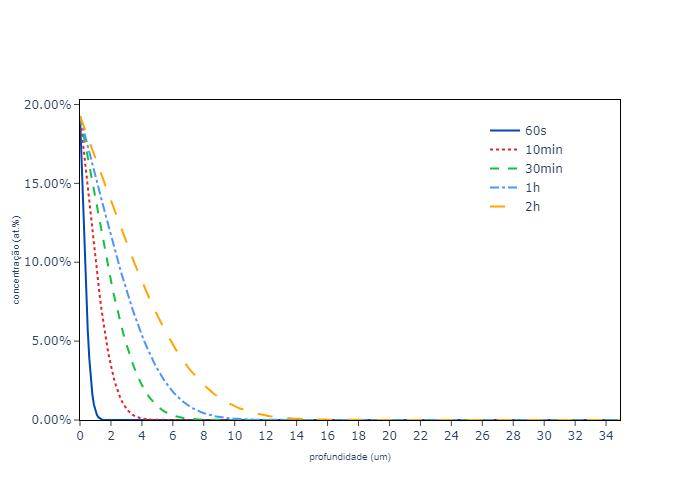
\includegraphics[width=1.0\textwidth]{plot_fickCte1}
	\label{fig:csvar-gas}
	\centering
	\fonte{Elaborado pela autora}
\end{figure}


\begin{figure}[ht]
\centering
	\caption{Resultado simulação para concentração na superfície constante até 22 horas}
	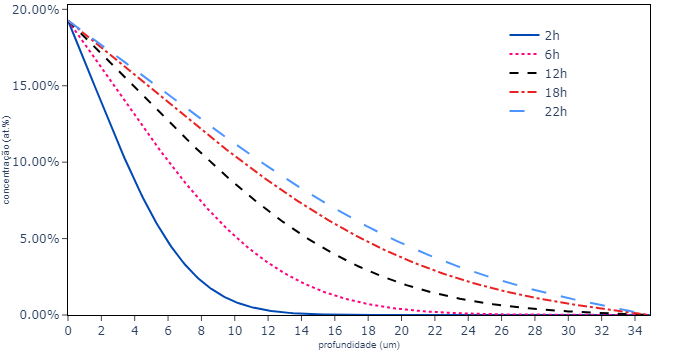
\includegraphics[width=1.0\textwidth]{plot_fickCte2}
	\label{fig:csvar-gas}
	\centering
	\fonte{Elaborado pela autora}
\end{figure}



\myworries{//escrever sobre os gráficos}

\subsection{Concentração na superfície variável}
\label{sec:modelo12}
Para simular a concentração na superfície durante nitretação gasosa de acordo com a descrição dada na Seção \autoref{sec:sol-numerica-2alei2}, foram utilizados os paramêtros dados pela \autoref{tab:parametros_csvar}.

\begin{table}[ht]
\centering
\setlength{\doublerulesep}{\arrayrulewidth}
{\def\arraystretch{2}\tabcolsep=10pt
\caption{Parâmetros para concentração na superfície variável nitretação gasosa}
\resizebox{\textwidth}{!}{
\begin{tabular}{c c c}
\hline\hline
Parâmetro & Descrição & Valor \\\hline
$\beta$ & Coeficiente para relacionar velocidade em que se atinge o equilíbrio & 0,0001 \\
$C_{eq}$ & Concentração de equilíbrio entre gás e aço &  47.318,64 mol/m$^3$ (2,0358 $\times$ 10$^{28}$ m$^-3$)    \\
\hline\hline
\end{tabular}
\label{tab:parametros_csvar}
}
}
\end{table}

Os valores da \autoref{tab:parametros_csvar} foram retirados de \cite{christiansen2008nitrogen}. O valor de $\beta$ foi definido testando o melhor \textit{fit} em dados experimentais e $C_{eq}$ foi definido como descrito na seção \autoref{sec:modelo11}.

Os resultados mostrando a concentração de nitrogênio em função da profundidade ao longo do tempo para a simulação com concentração superficial variável estão representados na Figura \ref{fig:csvar-gas}.

\begin{figure}[ht]
\centering
	\caption{Resultado simulação para concentração na superfície variável considerando nitretação a gás, até 2 horas}
	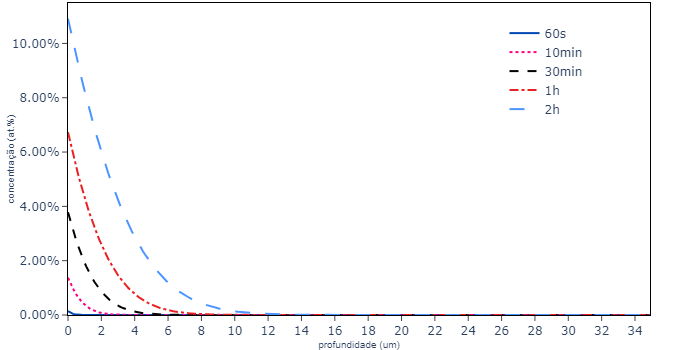
\includegraphics[width=1.0\textwidth]{plot_fickGas}
	\label{fig:csvar-gas}
	\centering
	\fonte{Elaborado pela autora}
\end{figure}

\begin{figure}[ht]
\centering
	\caption{Resultado simulação para concentração na superfície variável considerando nitretação a gás, até 22 horas}
	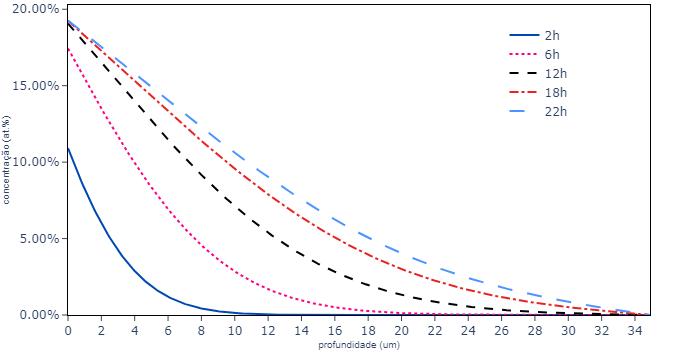
\includegraphics[width=1.0\textwidth]{plot_fickGas2}
	\label{fig:csvar-gas}
	\centering
	\fonte{Elaborado pela autora}
\end{figure}

\myworries{//escrever sobre os gráficos}

\myworries{//adicionar a plasma - para simular a plasma preciso de um j --> OK - arrumar e rodar (PC Lu)}

\section{Modelo 2 - \textit{Trapping-Detrapping}}
\subsection{Concentração na superfície constante}
\label{sec:modelo21}
\myworries{//apenas para um preview do tf - vou rodar para mais horas para a versao final}
\begin{figure}[ht]
\centering
	\caption{Resultado simulação para o modelo de \textit{trapping-detrapping} para concentração na superfície constante }
	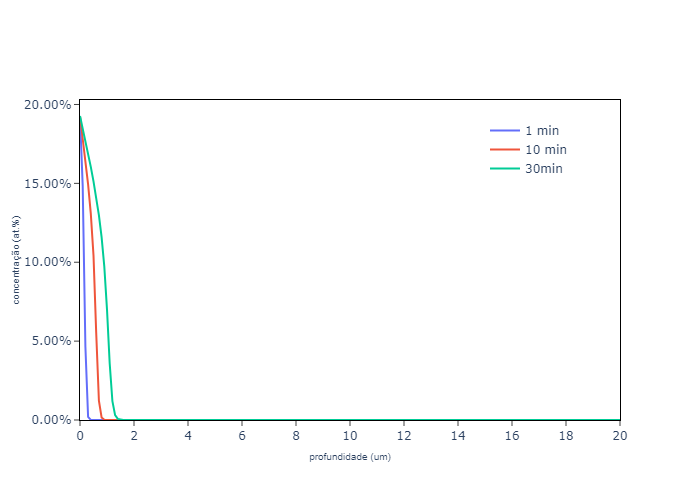
\includegraphics[width=8cm]{tmp-plot_trapDetrapGamma}
	\label{fig:csvar-gas}
	\centering
	\fonte{Elaborado pela autora}
\end{figure}


\begin{figure}[ht]
\centering
	\caption{Resultado simulação para o modelo de \textit{trapping-detrapping} para concentração na superfície constante - perfil do ndif e ntrap }
	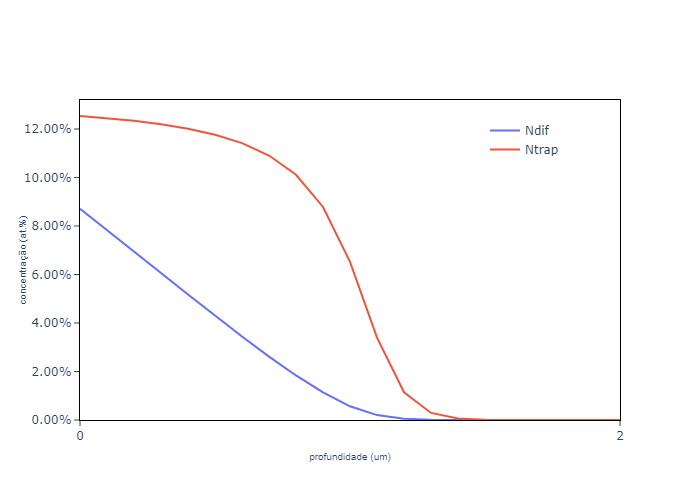
\includegraphics[width=8cm]{tmp-plot_trapDetrapCompGamma}
	\label{fig:csvar-gas}
	\centering
	\fonte{Elaborado pela autora}
\end{figure}

\subsection{Nitretação Gasosa}
\label{sec:modelo22}
\FloatBarrier
\myworries{definir qual escala vai ficar}

\myworries{rodando no meu pc}


A simulação para o modelo de \textit{trapping-detrapping} explicado na Seção \ref{sec:trap-detrap-gas-cc} com concentração da superfície dada pela condição de nitretação gasosa, utilizou os parâmetros mencionados na Seção \ref{params_sub}, os parâmetros para nitretação à gás da Seção \ref{sec:param-gas}, temperatura de 673K e os seguinte valores para a aplicação do método numérico:$\Delta t$ e $\Delta x$ utilizados foram 0,0001s e 0,1 $\mu m$, para um tempo total de \myworries{22 horas} e 20 $\mu m$ de profundidade.

Os resultados dessa simulação estão representados nas Figuras \ref{fig:td-csvar-gas} e \ref{fig:td-csvar-gas-both}, a primeira mostra o desenvolvimento do perfil de concentração de nitrogênio no tempo e a segunda mostra o perfil de concentração de nitrogênio livre, aprisionado e total após 2 horas.

\begin{figure}[ht]
\centering
	\caption{Resultado simulação para o modelo de \textit{trapping-detrapping} para nitretação gasosa, até 2 horas}
	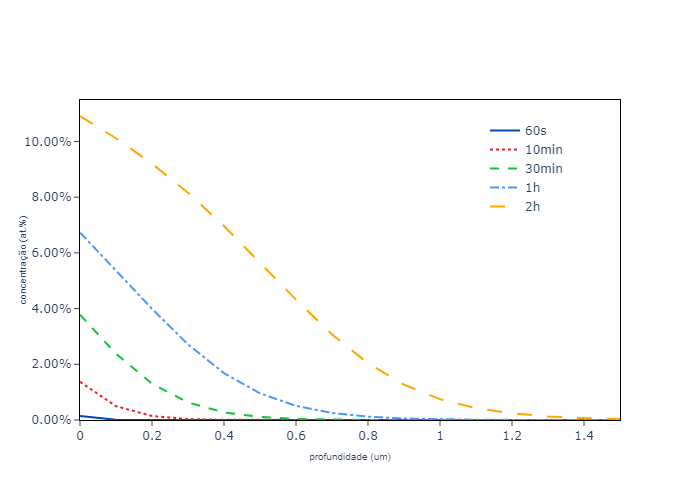
\includegraphics[width=1.0\textwidth]{plot_TrapDetrapGas_zoom}
	\label{fig:td-csvar-gas}
	\centering
	\fonte{Elaborado pela autora}
\end{figure}


\begin{figure}[ht]
\centering
	\caption{Resultado simulação para o modelo de \textit{trapping-detrapping} para nitreação gasosa - Perfil de Concentração de nitrogênio Livre e Aprisionado, após 2 horas }
	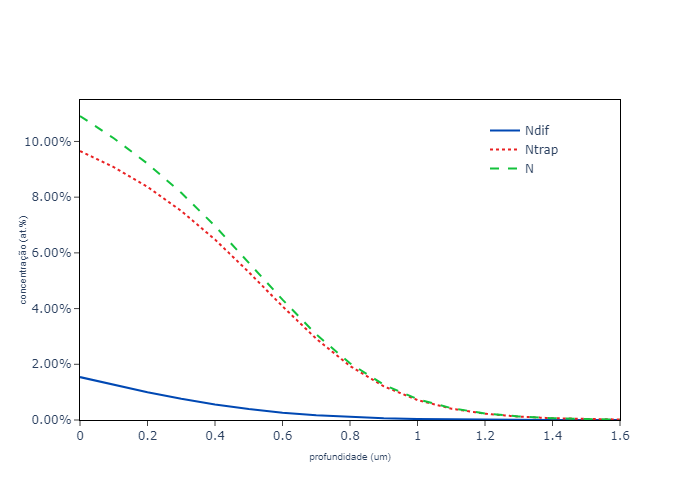
\includegraphics[width=1.0\textwidth]{plot_TrapDetrapGasBoth}
	\label{fig:td-csvar-gas-both}
	\centering
	\fonte{Elaborado pela autora}
\end{figure}

Na Figura \ref{fig:td-csvar-gas-compara}, foram plotadas ambas as soluções dos dois modelos estudados, para nitretação gasosa, mostrando o perfil de concentração de nitrogênio após 2 horas obtido para cada um.

\begin{figure}[ht]
\centering
	\caption{Resultado da simulação para os dois modelos considerando nitretação gasosa, após 2 horas }
	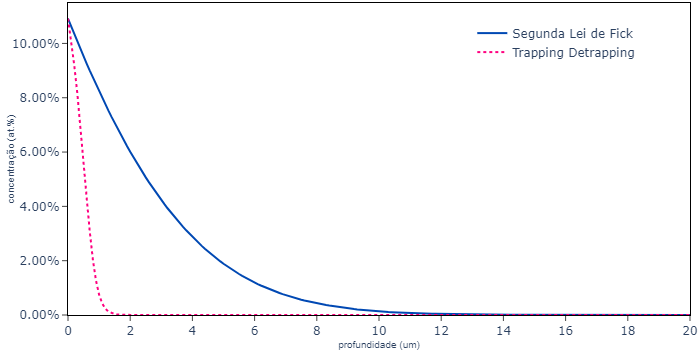
\includegraphics[width=1.0\textwidth]{plot_AmbosGas2h}
	\label{fig:td-csvar-gas-compara}
	\centering
	\fonte{Elaborado pela autora}
\end{figure}
\FloatBarrier

\subsection{Nitretação à Plasma}
\label{sec:modelo23}

\chapter{Discussão}
\section{Análise dos Resultados}
Os primeros resultados obtidos para a simulação da Segunda Lei de Fick estavam de acordo com o esperado como pode ser visto pelas figuras das Seção \ref{sec:modelo11}. As curvas de concentração de nitrogênio em função da profundidade apresentaram um comportamento exponencial, com seu valor máximo na superfície, diminuindo quanto maior a distânica da superfície e quanto maior o tempo, menor a inclinação da curva, esperado como um resultado do decorrer da difusão.

Para os resultados da Seção \ref{sec:modelo12}, na qual foi considerada que o efeito da nitretação gasosa na concentração superficial é que com o decorrer do tempo, a concentração tende àquela do equilíbrio, pode-se notar que o resultado obtido (ainda que correto conforme a Segunda Lei de Fick) não possui boa correlação com os resultados experimentais. Isso pode ser observado na Figura \ref{fig:csvar-gas2}, na qual para uma profundidade de aproximadamente 8$\mu m$ o perfil obtido experimentalmente apresenta uma queda brusca enquanto a solução dada pela Segunda Lei de Fick segue seu formato exponencial. Esse comportamento era esperado, dado que o pressuposto original era justamente que o mecanismo atuante na difusão do nitrogênio no aço não é dado pelo equacionamento de Fick. Como pode ser visto na Figura \ref{fig:csvar-gas2}, a concentração de nitrogênio para profundidades maiores que uma dada distância, apresentaram concentração inferior à esperada pela solução da equação de difusão de Fick. 

Esse comportamento pode estar associado ao aprisionamento do átomos de nitrogênio, dado que na ocorrência desse fenômeno o número de interstícios ocupados na camada superficial é maior, reduzindo assim a probabilidade de saltos e o fluxo de átomos, causando um atraso na propagação da difusão para dentro do material.

Para a nitretação à plasma aplicada à Segunda Lei de Fick visto na Seção \ref{sec:modelo22}, os valores obtidos para a concentração superficial superaram às obtidas pelo mesmo modelo considerando nitretação à gás, ainda que parecia convergir para um valor após algumas horas de simulação. O valor obtido na superfície, próximo de 40\%, superestimam também os valores encontrados na literatura para a conceentração de nitrogênio na austenita expandida - valor para o qual a possibilidade de precipitação deve ser considerada, outro motivo que não torna o resultado satisfatório para esse caso. Na Figura \ref{fig:csvar-plasma1}, os dados experimentais mostram uma penetração de nitrogênio para profundidades maiores do que mostram os resultados da simulação. Uma possível explicação para isso está na complexidade de modelar o processo de nitretação à plasma, pois este envolve diversos fatores que serão explorados em seguida.

\myworries{nenhuma simulacao de trapdetrap rodou ate 22 horas }

As simulações para o modelo de trapping-detrapping, apresentados na Seção \ref{sec:modelo2}, apresentaram o formato de curva esperado, no sentido que o perfil de concentração se inicia com uma leve inclinação, definida por uma região identificada normalmente como um platô, seguida de uma mudança brusca da inclinação indicando uma queda da concentração do átomo. Esse comportamento pode ser visto para a concentração superficial constante na Figura \ref{fig:td-cscte1}, para concentração superficial em caso de nitretação gasosa na Figura \ref{fig:td-csvar-gas}.

As Figuras \ref{fig:td-cscte-both} e \ref{fig:td-csvar-gas-both} mostram o perfil de nitrogênio livre, nitrogênio aprisionado e nitrogênio total após 2 horas, para concentração superficial constante e para nitretação gasosa, respectivamente. Nelas, observa-se que a concentração de nitrogênio em sítios de aprisionamentos é maior que a de nitrogênio livre e que a primeira possui uma queda mais brusca, enquanto a segunda possui um comportamento mais parecido com o da difusão clássica dada pela Segunda Lei de Fick. A somatória das duas concentrações resulta na curva com o comportamento conhecido da difusão de nitrogênio em aços, mencionada anteriormente. Destaca-se que os resultados estão dentro do esperado pois o comportamento observado é o mesmo que foi obtido pelo modelo de Galdikas e Moskalioviene em \cite{moskalioviene2011modeling}. 

As Figuras \ref{fig:td-cscte-compara} e \ref{fig:td-csvar-gas-compara} mostram como o perfil de concentração obtido se diferencia da Segunda Lei de Fick, principalmente devido ao platô no próximo da superfície.

\myworries{As profundidades obtidas estão de acordo com o esperado... -> para 22 horas (cs cte ou/e gas }

Para a duração de 2 horas, os resultados obtidos para o perfil de concentração de nitrogênio no modelo de \textit{trapping-detrapping} considerando nitretação à plasma subestimou a concentração real obtida por \cite{moskalioviene2011modeling} como visto na Figura \myworries{colocar figura quando tiver}. Pode-se notar que nenhum modelo obteve valores próximos daqueles obtidos por Moskalioviene e Galdikas para um intervalo de tempo pequeno como 2 horas. Possíveis explicações estão nas características do processo que não foram levadas em contas no modelo desse trabalho e também devido à simplificações feitas ao modelo, que serão discutidas na Seção \ref{sec:discussao}.

Uma simplificação feita para a simulação do modelo de \textit{trapping-detrapping} desse trabalho foi a omissão do fator 4$\pi$ dos coeficientes de \textit{trapping} e  \textit{detrapping}. Essa escolha pode ter trazido diferenças na velocidade com que a difusão ocorre para dentro do material, provocando divergências quando comparadas com outros resultados encontrados na literatura.

Com relação ao processo utilizado no artigo de Moskalioviene e Galdikas, observa-se que a nitretação à plasma foi feita sem a realização de sputtering na superfície. Segundo os autores a energia de aceleração dos íons utilizada foi inferior a 15 eV, que é menor que o limite de sputtering para a maioria dos materiais. Devido à ausência de sputtering, observou-se um aumento de volume, para o qual foi medido uma taxa relativa a esse processo (chamado de \textit{swelling}). Para considerar os efeitos desse fenômeno, os autores optaram por adicionar um termo de \textit{swelling} ao modelo, o qual não foi considerado para a realização do modelo no trabalho em questão, logo pode representar mais uma fonte de divergência.

\section{Discussão}
\label{sec:discussao}

Os principais fatores levados em consideração nos estudos da difusão do nitrogênio nos aços são a afinidade do cromo (que provoca o fenômeno de \textit{trapping-detrapping}, as tensões residuais, os efeitos de sputtering do processo à plasma, efeitos das reações na superfície e a dependência do coeficiente de difusão com a concentração.

Dessa forma o modelo desenvolvido possui algumas limitações, seguem algumas delas. Ele não pode ser utilizado para processos de nitretação com temperaturas superiores à 450°C, pois para tais temperaturas existe a possibilidade de precipitação de nitretos de cromo que não estão previstas no modelo. Não foram levadas em consideração os efeitos da taxa de sputtering e do surgimento de defeitos causados pelo bombardeamento de íon de alta energia no processo à plasma ou similiares. Não foram consideradas possíveis reações na superfície durante os processos de nitretação. Não foi analisado a influência de tensões causadas pela expansão do reticulado durante a incorporação de nitrogênio e não considerou-se a influência da composição no coeficiente de difusão.


\chapter{Conclusões}
\myworries{\textit{TO DO}}


% ========== Referências ==========
% --- ABNT (requer ABNTeX 2) ---
%	http://www.ctan.org/tex-archive/macros/latex/contrib/abntex2
\bibliographystyle{abntex2-alf}
\bibliography{references}


\chapter*{Anexos}
\myworries{anexos}
\section*{ANEXO A - Entradas das simulações}

\myworries{talvez a gte queira rodar de novo com coisas mais proximas do Somers}

\begin{table}[ht]
\centering
\setlength{\doublerulesep}{\arrayrulewidth}
{\def\arraystretch{2}\tabcolsep=10pt
\caption{Parâmetros para a simulação da Seção \ref{sec:modelo11} - Segunda Lei de Fick com concentração superficial constante}
\resizebox{\textwidth}{!}{
\begin{tabular}{c c c}
\hline\hline
Parâmetro & Descrição & Valor \\\hline
$C_{s}$   & Concentração na superfífice                & $47.318,64 mol/m^3 (2,0358 \times 10^{28} m^-3$) \\
$T$       & Temperatura                                & $718K$   \\
$E_A$     & Energia de ativação de Difusão             & $1,7622 \times 10^{-19} J$  \\
$D_0$     & Fator pré-exponencial de difusão           & $8,37 \times 10^{-8} m^2/s$  \\
$k_B$     & Constante de Boltzmann                     & $1,38064852 \times 10^{-23} J/K$ \\
$dt$      & Passo no tempo                             & $0,01s$ \\
$dx$      & Passo no espaço                            & $0,1 \mu s$ \\
$T$       & Intervalo de tempo da simulação            & $22 horas$ \\
$n$       & Profundidade total da simulação            & $35 \mu s$ \\
\hline\hline
\end{tabular}
\label{tab:parametros_modelo11}
}
}
\end{table}


\begin{table}[ht]
\centering
\setlength{\doublerulesep}{\arrayrulewidth}
{\def\arraystretch{2}\tabcolsep=10pt
\caption{\myworries{tabela Fick Gas} Parâmetros para a simulação da Seção \ref{sec:modelo12} - Segunda Lei de Fick com nitretação gasosa}
\resizebox{\textwidth}{!}{
\begin{tabular}{c c c}
\hline\hline
Parâmetro & Descrição & Valor \\\hline
$C_{eq}$   & Concentração de equilíbrio                & $47.318,64 mol/m^3 (2,0358 \times 10^{28} m^-3$) \\
$T$       & Temperatura                                & $718K$   \\
$E_A$     & Energia de ativação de Difusão             & $1,7622 \times 10^{-19} J$  \\
$D_0$     & Fator pré-exponencial de difusão           & $8,37 \times 10^{-8} m^2/s$  \\
$k_B$     & Constante de Boltzmann                     & $1,38064852 \times 10^{-23} J/K$ \\
$\beta$   & Coeficiente de relação de alcance do equilíbrio   & $0,0001$ \\
$dt$      & Passo no tempo                             & $0,01s$ \\
$dx$      & Passo no espaço                            & $0,1 \mu s$ \\
$T$       & Intervalo de tempo da simulação            & $22 horas$ \\
$n$       & Profundidade total da simulação            & $35 \mu s$ \\
\hline\hline
\end{tabular}
\label{tab:parametros_modelo121}
}
}
\end{table}


\begin{table}[ht]
\centering
\setlength{\doublerulesep}{\arrayrulewidth}
{\def\arraystretch{2}\tabcolsep=10pt
\caption{\myworries{tabela Fick Plasma} Parâmetros para a simulação da Seção \ref{sec:modelo12} - Segunda Lei de Fick com nitretação à plasma}
\resizebox{\textwidth}{!}{
\begin{tabular}{c c c}
\hline\hline
Parâmetro & Descrição & Valor \\\hline
$T$       & Temperatura                                & $673 K$   \\
$E_A$     & Energia de ativação de Difusão             & $1,7622 \times 10^{-19} J$  \\
$D_0$     & Fator pré-exponencial de difusão           & $8,37 \times 10^{-8} m^2/s$  \\
$k_B$     & Constante de Boltzmann                     & $1,38064852 \times 10^{-23} J/K$ \\
$H_0$     & Concentração de Átomos Hospedeiros         & $H_0 = 7,29 \times 10^{28} m^{-3}$ \\
$H_{superfície}$     & Concentração de Átomos Hospedeiros na superfície & $H_{superfície} = 8 \times 10^{25} m^{-2}$ \\
$\alpha$  & Coeficiente de adesão do nitrogênio nos componentes   & $1$ \\
$j$       & Densidade de corrente média   & $4,4 A/m^2$ \\
$q$       & Carga elementar   & $1,602\times 10^{-19}C$ \\
$dt$      & Passo no tempo                             & $0,01s$ \\
$dx$      & Passo no espaço                            & $0,1 \mu s$ \\
$T$       & Intervalo de tempo da simulação            & $22 horas$ \\
$n$       & Profundidade total da simulação            & $20 \mu s$ \\
\hline\hline
\end{tabular}
\label{tab:parametros_modelo122}
}
}
\end{table}


\begin{table}[ht]
\centering
\setlength{\doublerulesep}{\arrayrulewidth}
{\def\arraystretch{2}\tabcolsep=10pt
\caption{\myworries{tabela Trap Detrap Cte} Parâmetros para a simulação da Seção \ref{sec:modelo21} - \textit{Trapping-Detrapping} com concentração constante}
\resizebox{\textwidth}{!}{
\begin{tabular}{c c c}
\hline\hline
Parâmetro & Descrição & Valor \\\hline
$C_{s}$   & Concentração na superfífice                & $47.318,64 mol/m^3 (2,0358 \times 10^{28} m^-3$) \\
$T$       & Temperatura                                & $673 K$   \\
$E_A$     & Energia de ativação de Difusão             & $1,7622 \times 10^{-19} J$  \\
$E_B$     & Energia de ativação de \textit{detrapping}             & $4,48609 \times 10^{-20} J$  \\
$R_t$     & Raio de aprisionamento                     & $0,38 \times 10^{-9} m$  \\
$D_0$     & Fator pré-exponencial de difusão           & $8,37 \times 10^{-8} m^2/s$  \\
$k_B$     & Constante de Boltzmann                     & $1,38064852 \times 10^{-23} J/K$ \\
$H_0$     & Concentração de Átomos Hospedeiros         & $H_0 = 7,29 \times 10^{28} m^{-3}$ \\
$H_t$     & Concentração de Sítios de Aprisionamento         & $H_t = 1,31 \times 10^{28} m^{-3}$ \\
$dt$      & Passo no tempo                             & $0,0001s$ \\
$dx$      & Passo no espaço                            & $0,1 \mu s$ \\
$T$       & Intervalo de tempo da simulação            & $22 horas$ \\
$n$       & Profundidade total da simulação            & $20 \mu s$ \\
\hline\hline
\end{tabular}
\label{tab:parametros_modelo21}
}
}
\end{table}


\begin{table}[ht]
\centering
\setlength{\doublerulesep}{\arrayrulewidth}
{\def\arraystretch{2}\tabcolsep=10pt
\caption{\myworries{tabela Trap Detrap Gas} Parâmetros para a simulação da Seção \ref{sec:modelo21} - \textit{Trapping-Detrapping} com nitretação gasosa}
\resizebox{\textwidth}{!}{
\begin{tabular}{c c c}
\hline\hline
Parâmetro & Descrição & Valor \\\hline
$C_{eq}$  & Concentração de equilíbrio                 & $47.318,64 mol/m^3 (2,0358 \times 10^{28} m^-3$) \\
$T$       & Temperatura                                & $673 K$   \\
$E_A$     & Energia de ativação de Difusão             & $1,7622 \times 10^{-19} J$  \\
$E_B$     & Energia de ativação de \textit{detrapping} & $4,48609 \times 10^{-20} J$  \\
$R_t$     & Raio de aprisionamento                     & $0,38 \times 10^{-9} m$  \\
$D_0$     & Fator pré-exponencial de difusão           & $8,37 \times 10^{-8} m^2/s$  \\
$k_B$     & Constante de Boltzmann                     & $1,38064852 \times 10^{-23} J/K$ \\
$H_0$     & Concentração de Átomos Hospedeiros         & $H_0 = 7,29 \times 10^{28} m^{-3}$ \\
$H_t$     & Concentração de Sítios de Aprisionamento   & $H_t = 1,31 \times 10^{28} m^{-3}$ \\
$H_{superfície}$     & Concentração de Átomos Hospedeiros na superfície & $H_{superfície} = 8 \times 10^{25} m^{-2}$ \\
$\beta$   & Coeficiente de relação de alcance do equilíbrio   & $0,0001$ \\
$dt$      & Passo no tempo                             & $0,0001s$ \\
$dx$      & Passo no espaço                            & $0,1 \mu s$ \\
$T$       & Intervalo de tempo da simulação            & $22 horas$ \\
$n$       & Profundidade total da simulação            & $20 \mu s$ \\
\hline\hline
\end{tabular}
\label{tab:parametros_modelo221}
}
}
\end{table}


\begin{table}[ht]
\centering
\setlength{\doublerulesep}{\arrayrulewidth}
{\def\arraystretch{2}\tabcolsep=10pt
\caption{\myworries{tabela Trap Detrap Plasma} Parâmetros para a simulação da Seção \ref{sec:modelo21} - Segunda Lei de Fick com nitretação à plasma}
\resizebox{\textwidth}{!}{
\begin{tabular}{c c c}
\hline\hline
Parâmetro & Descrição & Valor \\\hline
$C_{s}$   & Concentração na superfífice                & $47.318,64 mol/m^3 (2,0358 \times 10^{28} m^-3$) \\
$T$       & Temperatura                                & $673 K$   \\
$E_A$     & Energia de ativação de Difusão             & $1,7622 \times 10^{-19} J$  \\
$E_B$     & Energia de ativação de \textit{detrapping}             & $4,48609 \times 10^{-20} J$  \\
$R_t$     & Raio de aprisionamento                     & $0,38 \times 10^{-9} m$  \\
$D_0$     & Fator pré-exponencial de difusão           & $8,37 \times 10^{-8} m^2/s$  \\
$k_B$     & Constante de Boltzmann                     & $1,38064852 \times 10^{-23} J/K$ \\
$H_0$     & Concentração de Átomos Hospedeiros         & $H_0 = 7,29 \times 10^{28} m^{-3}$ \\
$H_t$     & Concentração de Sítios de Aprisionamento         & $H_t = 1,31 \times 10^{28} m^{-3}$ \\
$H_{superfície}$     & Concentração de Átomos Hospedeiros na superfície & $H_{superfície} = 8 \times 10^{25} m^{-2}$ \\
$\alpha$  & Coeficiente de adesão do nitrogênio nos componentes   & $1$ \\
$j$       & Densidade de corrente média   & $4,4 A/m^2$ \\
$q$       & Carga elementar   & $1,602\times 10^{-19}C$ \\
$dt$      & Passo no tempo                             & $0,01s$ \\
$dx$      & Passo no espaço                            & $0,1 \mu s$ \\
$T$       & Intervalo de tempo da simulação            & $22 horas$ \\
$n$       & Profundidade total da simulação            & $20 \mu s$ \\
\hline\hline
\end{tabular}
\label{tab:parametros_modelo222}
}
}
\end{table}



\myworries{. colocar tabela da funcao erro nos anexos}
\myworries{. colocar os códigos}


\end{document}